\subsection{Matching Of Impedances}\label{lec:lec12}
In previous sections, we have dealt with other applications of transmission lines. In this section, we will discuss the most important application of transmission lines, which is \emph{\textquotedblleft Impedance Matching\textquotedblright}\index{impedance matching}.

As we know when the load impedance is equal to characteristic impedance $Z_0$, there is no reflection on the line, hence there is maximum power transfer. But this \textit{matching condition}\index{matching condition} is not always feasible. Thus, we need a module or device which will transform the load impedance to the characteristic impedance. This module is known as a \textbf{matching transformer unit}\index{matching transformer} as shown in figure~\ref{fig:fig7}.
\begin{figure}[h]
\centering
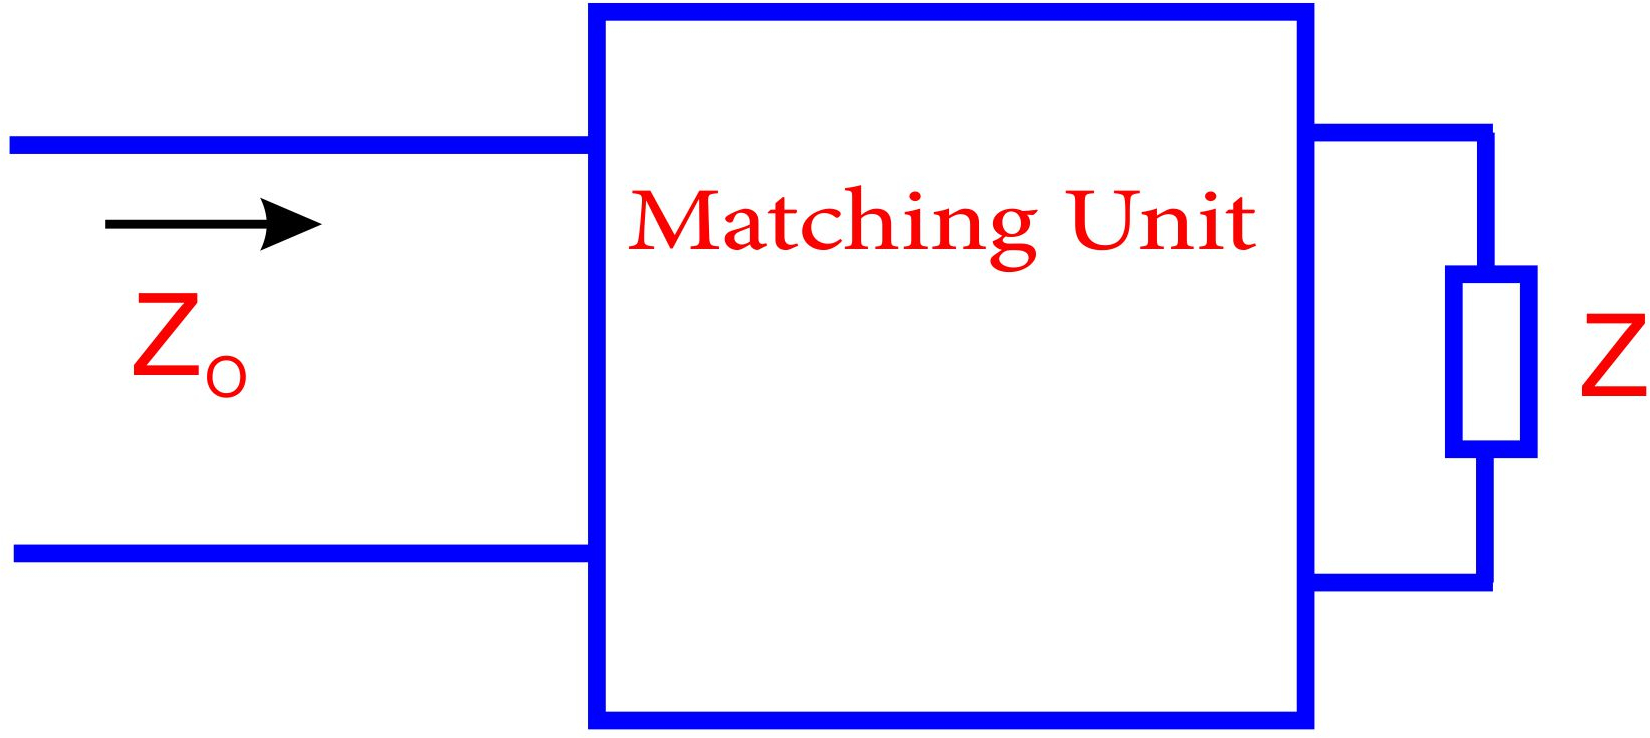
\includegraphics[width=0.7\linewidth]{\pathtopartone/graphics/fig7}
\caption{Matching Transformer unit}
\label{fig:fig7}
\end{figure} 

Let us suppose we want to convert the output impedance $Z$ with the matching unit (transformer) to the characteristic impedance $Z_0$, which is shown in figure~\ref{fig:fig7}. At the input (leftmost side), we should see a characteristic impedance $ Z_0$ and the module should be completely lossless (ideal) to allow maximum power transfer to load $Z$. First, let us discuss various methods by which different impedances can be matched to the characteristic impedance.
\begin{figure}[h]
\centering
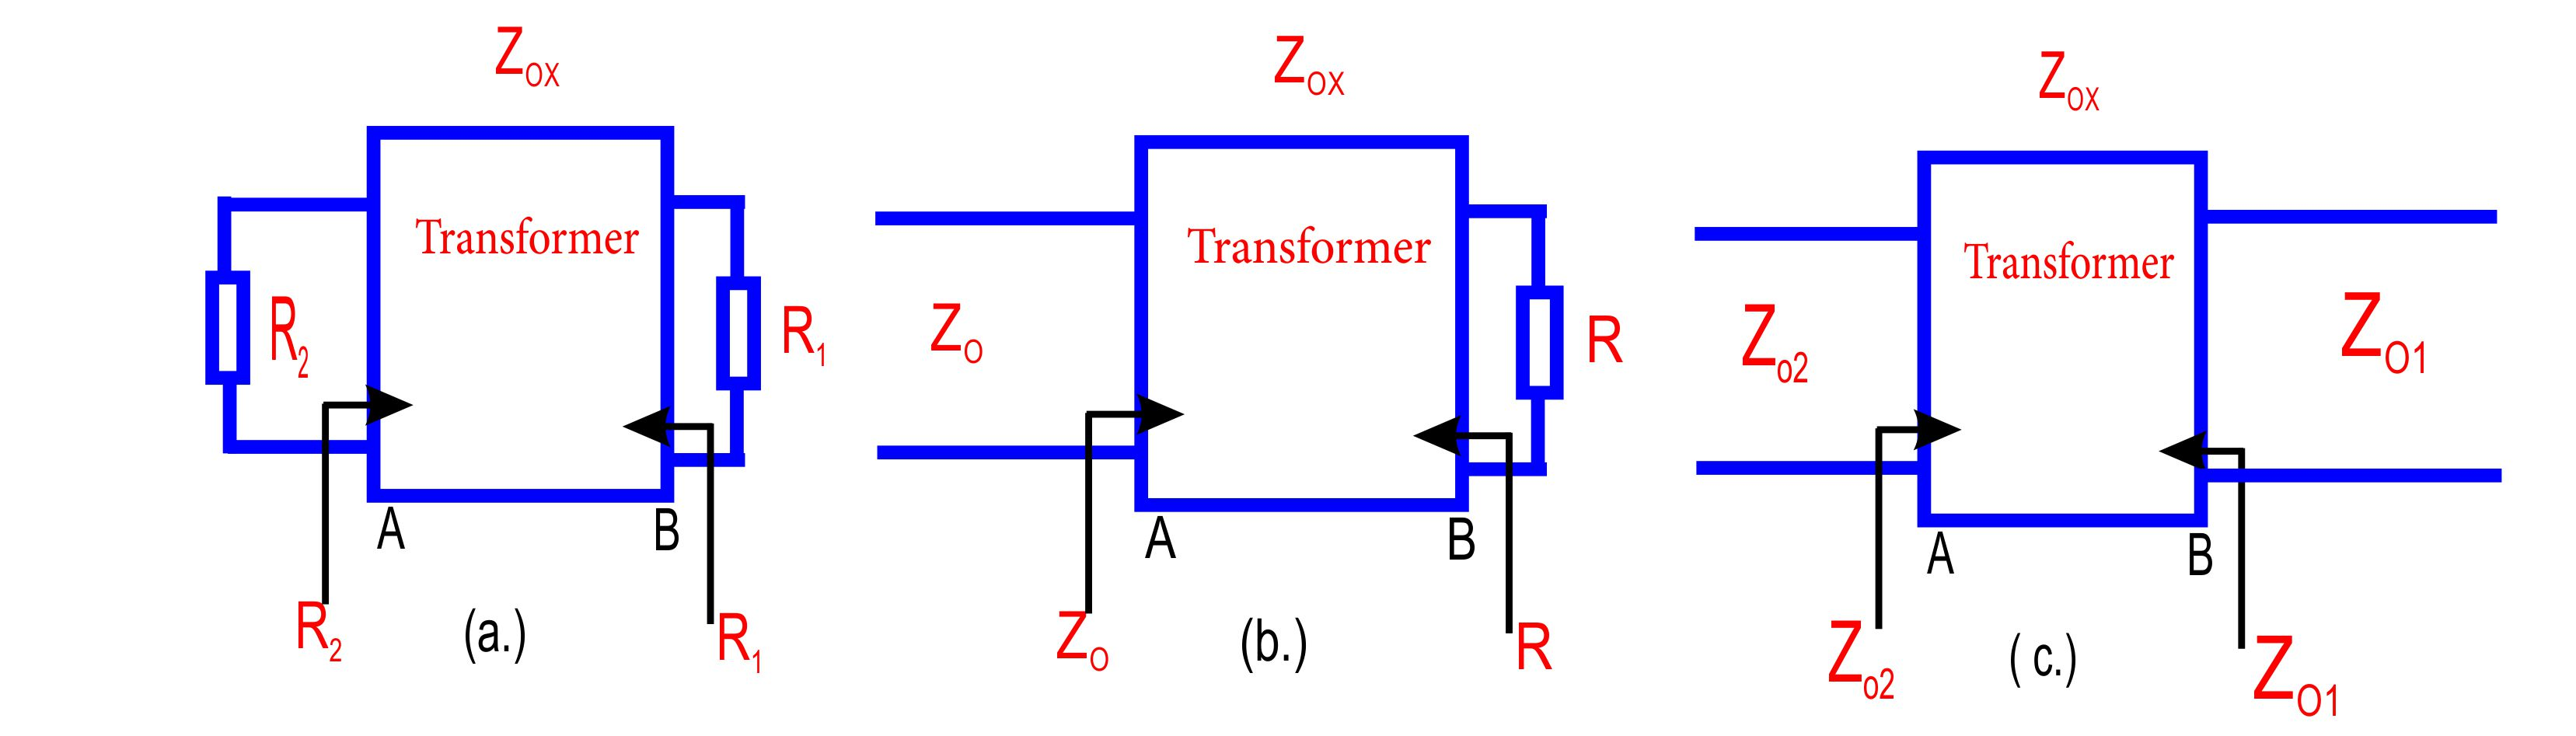
\includegraphics[width=1\linewidth]{\pathtopartone/graphics/fig8}
\caption{Application of transformer}
\label{fig:fig8}
\end{figure}

In figure~{\ref{fig:fig8}a} we have two different resistances $R_1$ and $R_2$ which are to be matched, that is, $R_1\neq R_2$. If they are connected directly there will be a mismatch and no maximum power transfer from $R_1$ to $R_2$. We then introduce some device in between that will make $R_1$ appear like $R_2$ when seen from the left side and $R_2$ appear like $R_1$, when seen from the right side, so from both sides it will appear that they are matched to the load and there is maximum power transfer. In figure~\ref{fig:fig8}b, we are matching R to $Z_0$, and like the previous case study we place in a module to match the impedances between R and $Z_0$. Hence on the left side, we should see $Z_0$ and vice versa. lastly, in figure~{\ref{fig:fig8}c}, which is the most important case. We have two long transmission lines which are to be connected together. If the length of each transmission is very large, the input impedance of transmission line one (1) will appear as its characteristics impedance $ Z_{01}$ and transmission line two (2) will appear as its characteristics impedance $ Z_{02}$. For maximum power transfer, we bring a transforming device in between that will make $Z_{01}$ see $Z_{02}$ as $Z_{01}$ and vice-versa. From both sides, it seems as if the line is terminated in its characteristic impedance. Hence there will be no reflection on either side of the transmission line.

\subsubsection{Quarter Wavelength Transformer Technique}
On the Smith Chart, if we have an impedance which is resistive, \emph{how much can we move on the transmission line so that the impedance always appears like a resistance?} Let us introduce some section of the transmission line in between both impedances (input and output) which has a characteristic impedance $ Z_{0x}$ in figure~{\ref{fig:fig8}a} and~\ref{fig:fig8}b and is different from the characteristic impedance $ Z_0$ to which the resistive impedance R is to be matched.

Hence, we find out $ Z_{0x}$ and the length of this introduced transmission line for which R can be matched with $ Z_0$. Resistive impedance lie on the horizontal axis of the Smith Chart, $Z > Z_0$ lies on the right and $Z < Z_0$ lies on the left of the Smith chart. So the question is, \emph{what should be the value of $Z_{0x}$ and length $l$, that will match the resistive impedance to the characteristic impedance $Z_0$?} From the Smith Chart, to transform from $R$ to another resistive value, we need to move by either $ \frac{\lambda}{4}$ or $ \frac{\lambda}{2}$. But a $\frac{\lambda}{2}$ movement brings us back to the same impedance and thus we don't use this value because it will transform the impedance to itself. A $\frac{\lambda}{4}$ movement on the other hand, will have a resistive impedance which is different from the original resistive impedance(that is, inverts itself), thus $l = \frac{\lambda}{4} $ will be most appropriate because at this length we will have a different resistive value.
\begin{figure}[h]
\centering
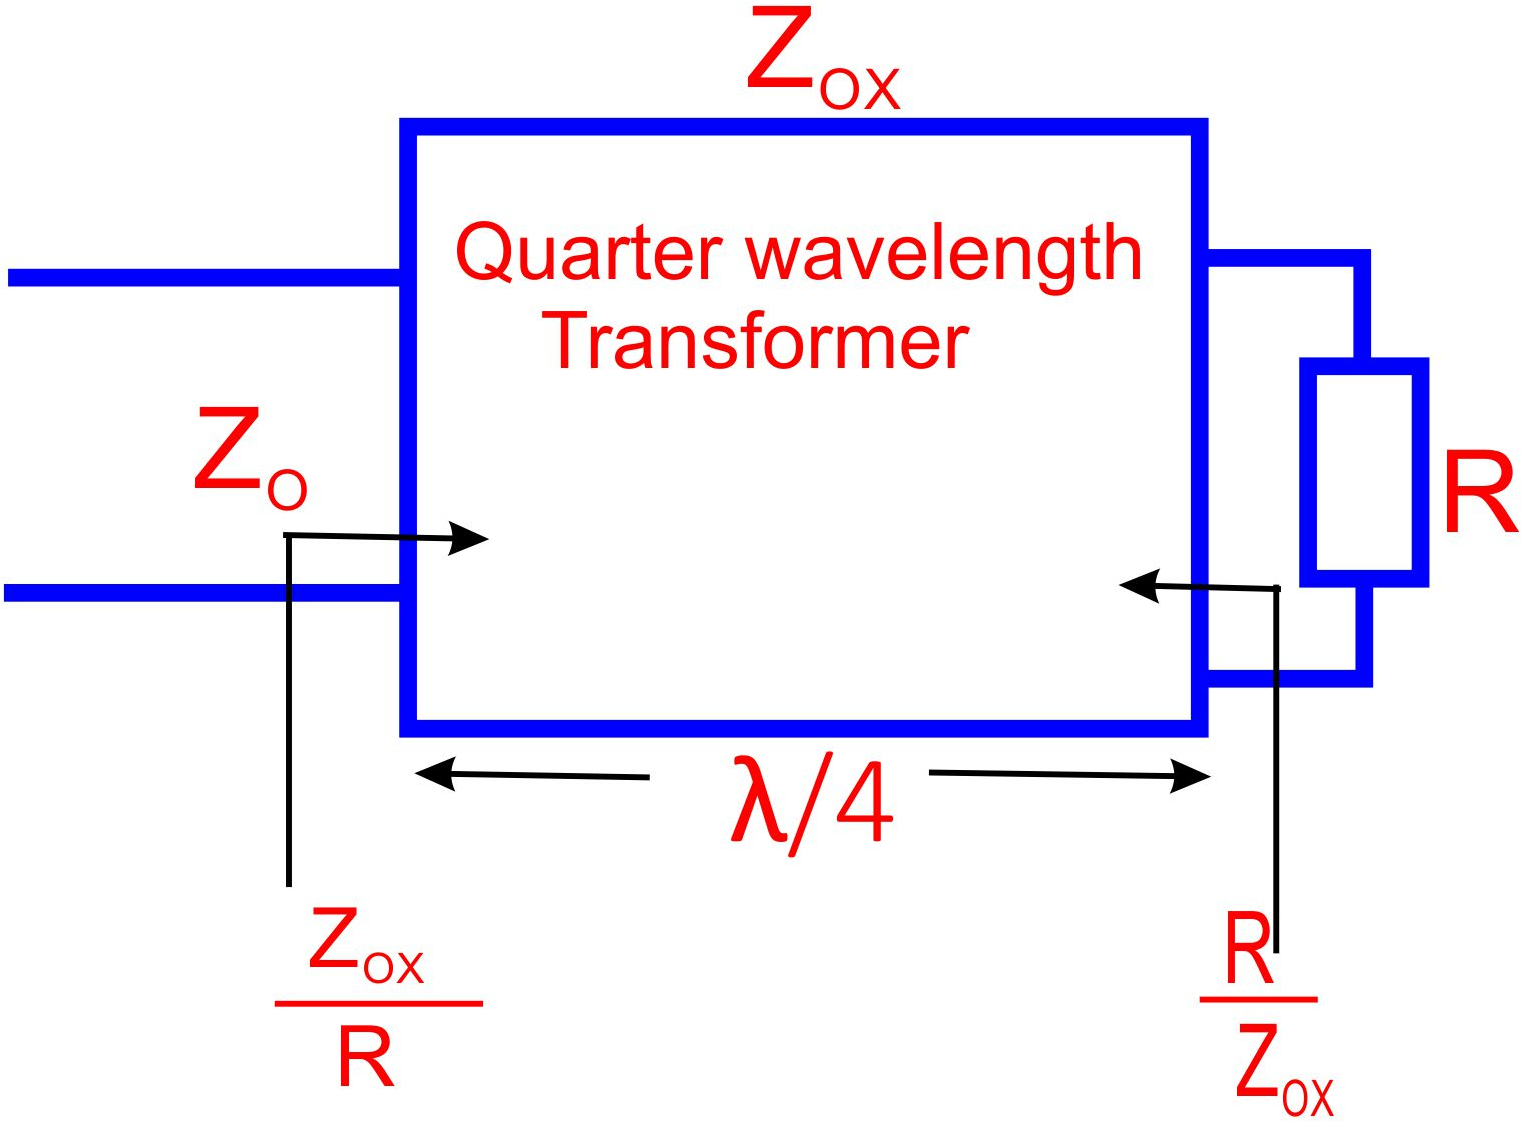
\includegraphics[width=0.7\linewidth]{\pathtopartone/graphics/fig9}
\caption{The quarter wavelength transformer technique}
\label{fig:fig9}
\end{figure}

From figure~\ref{fig:fig9}, at the transformer (output), the normalised impedance seen will be $\frac{R}{Z_{0x}}$. At the transformer (input), the normalised impedance seen will be $\frac{Z_{0x}}{R}$\footnote{
We know from the property of the transmission line, that for every distance of $l = \frac{\lambda}{4}$, the impedance inverts itself
}. So the absolute characteristic impedance $ Z_0$ seen at the input will be equal to: 
\begin{dmath*}
Z_0=\left(\frac{Z_{0x}}{R}\right)\times Z_{0x}
=\frac{Z_{0x}^2}{R}
\end{dmath*}
Therefore,
\begin{equation}
Z_{0x}=\sqrt{RZ_0}
\label{eqn:xteristicsimptransformer}
\end{equation}
Equation~\eqref{eqn:xteristicsimptransformer} implies that if we have a mismatch condition, we can input a matching transformer (an example is the \uppercase{balun}\footnote{
A \uppercase{balun} is a type of electrical transformer used to connect a balanced transmission line, such as a twisted pair cable, to an unbalanced transmission line, such as a coaxial cable. The name \uppercase{balun} is short for \textquotedblleft\;balanced to unbalanced.\textquotedblright\;. It has a length $l=\frac{\lambda}{4}$, and a characteristic impedance $Z_{0x}$. \uppercase{Balun}s are commonly used in radio and television systems, as well as in data communication networks. They are available in a variety of designs, including ferrite-core \uppercase{balun}s, air-core \uppercase{balun}s, and transmission line \uppercase{balun}s.
}\index{balun}). Introducing this section of the transmission line, we will have a matched condition where R will appear as $ Z_0$ when seen from the input and $ Z_0$ will appear as R when seen from the output. Since the transmission line is lossless, there is a match on the transmission line from $ Z_0$ to R, therefore, we will see a maximum power transfer.
This technique of matching impedance is known as the \textbf{Quarter Wavelength Transformer Technique}\index{quarter wavelength transformer technique} which derives its name from the fact that we have to travel a length which is equal to a quarter, that is, 1/4 of the wavelength $\lambda$. This matching transformer is also used for matching lumped circuits.

\subsubsection{Complex Load Impedance Matching}
Now, we would like to find out \emph{can the technique (quarter wavelength transformer technique) only be used to match resistive impedance?} The answer is no, we can use this method to solve complex impedances but it requires us to do some thinking because, at first look, it appears impossible. This is because on the Smith Chart, to derive $Z_{0x}$, we use only the horizontal axis of the chart. Now, \emph{how can we use both the real and imaginary parts of the chart?}

We solve it by first transforming the complex normalized impedances to a real impedance. This is done by moving along the length of a transmission line. That means if you introduce some length of transmission line with characteristic impedance $ Z_0$, then the impedance seen at the other end is real if the length is such that you get a voltage (maximum or minimum) for that length.
\begin{figure}[h]
\centering
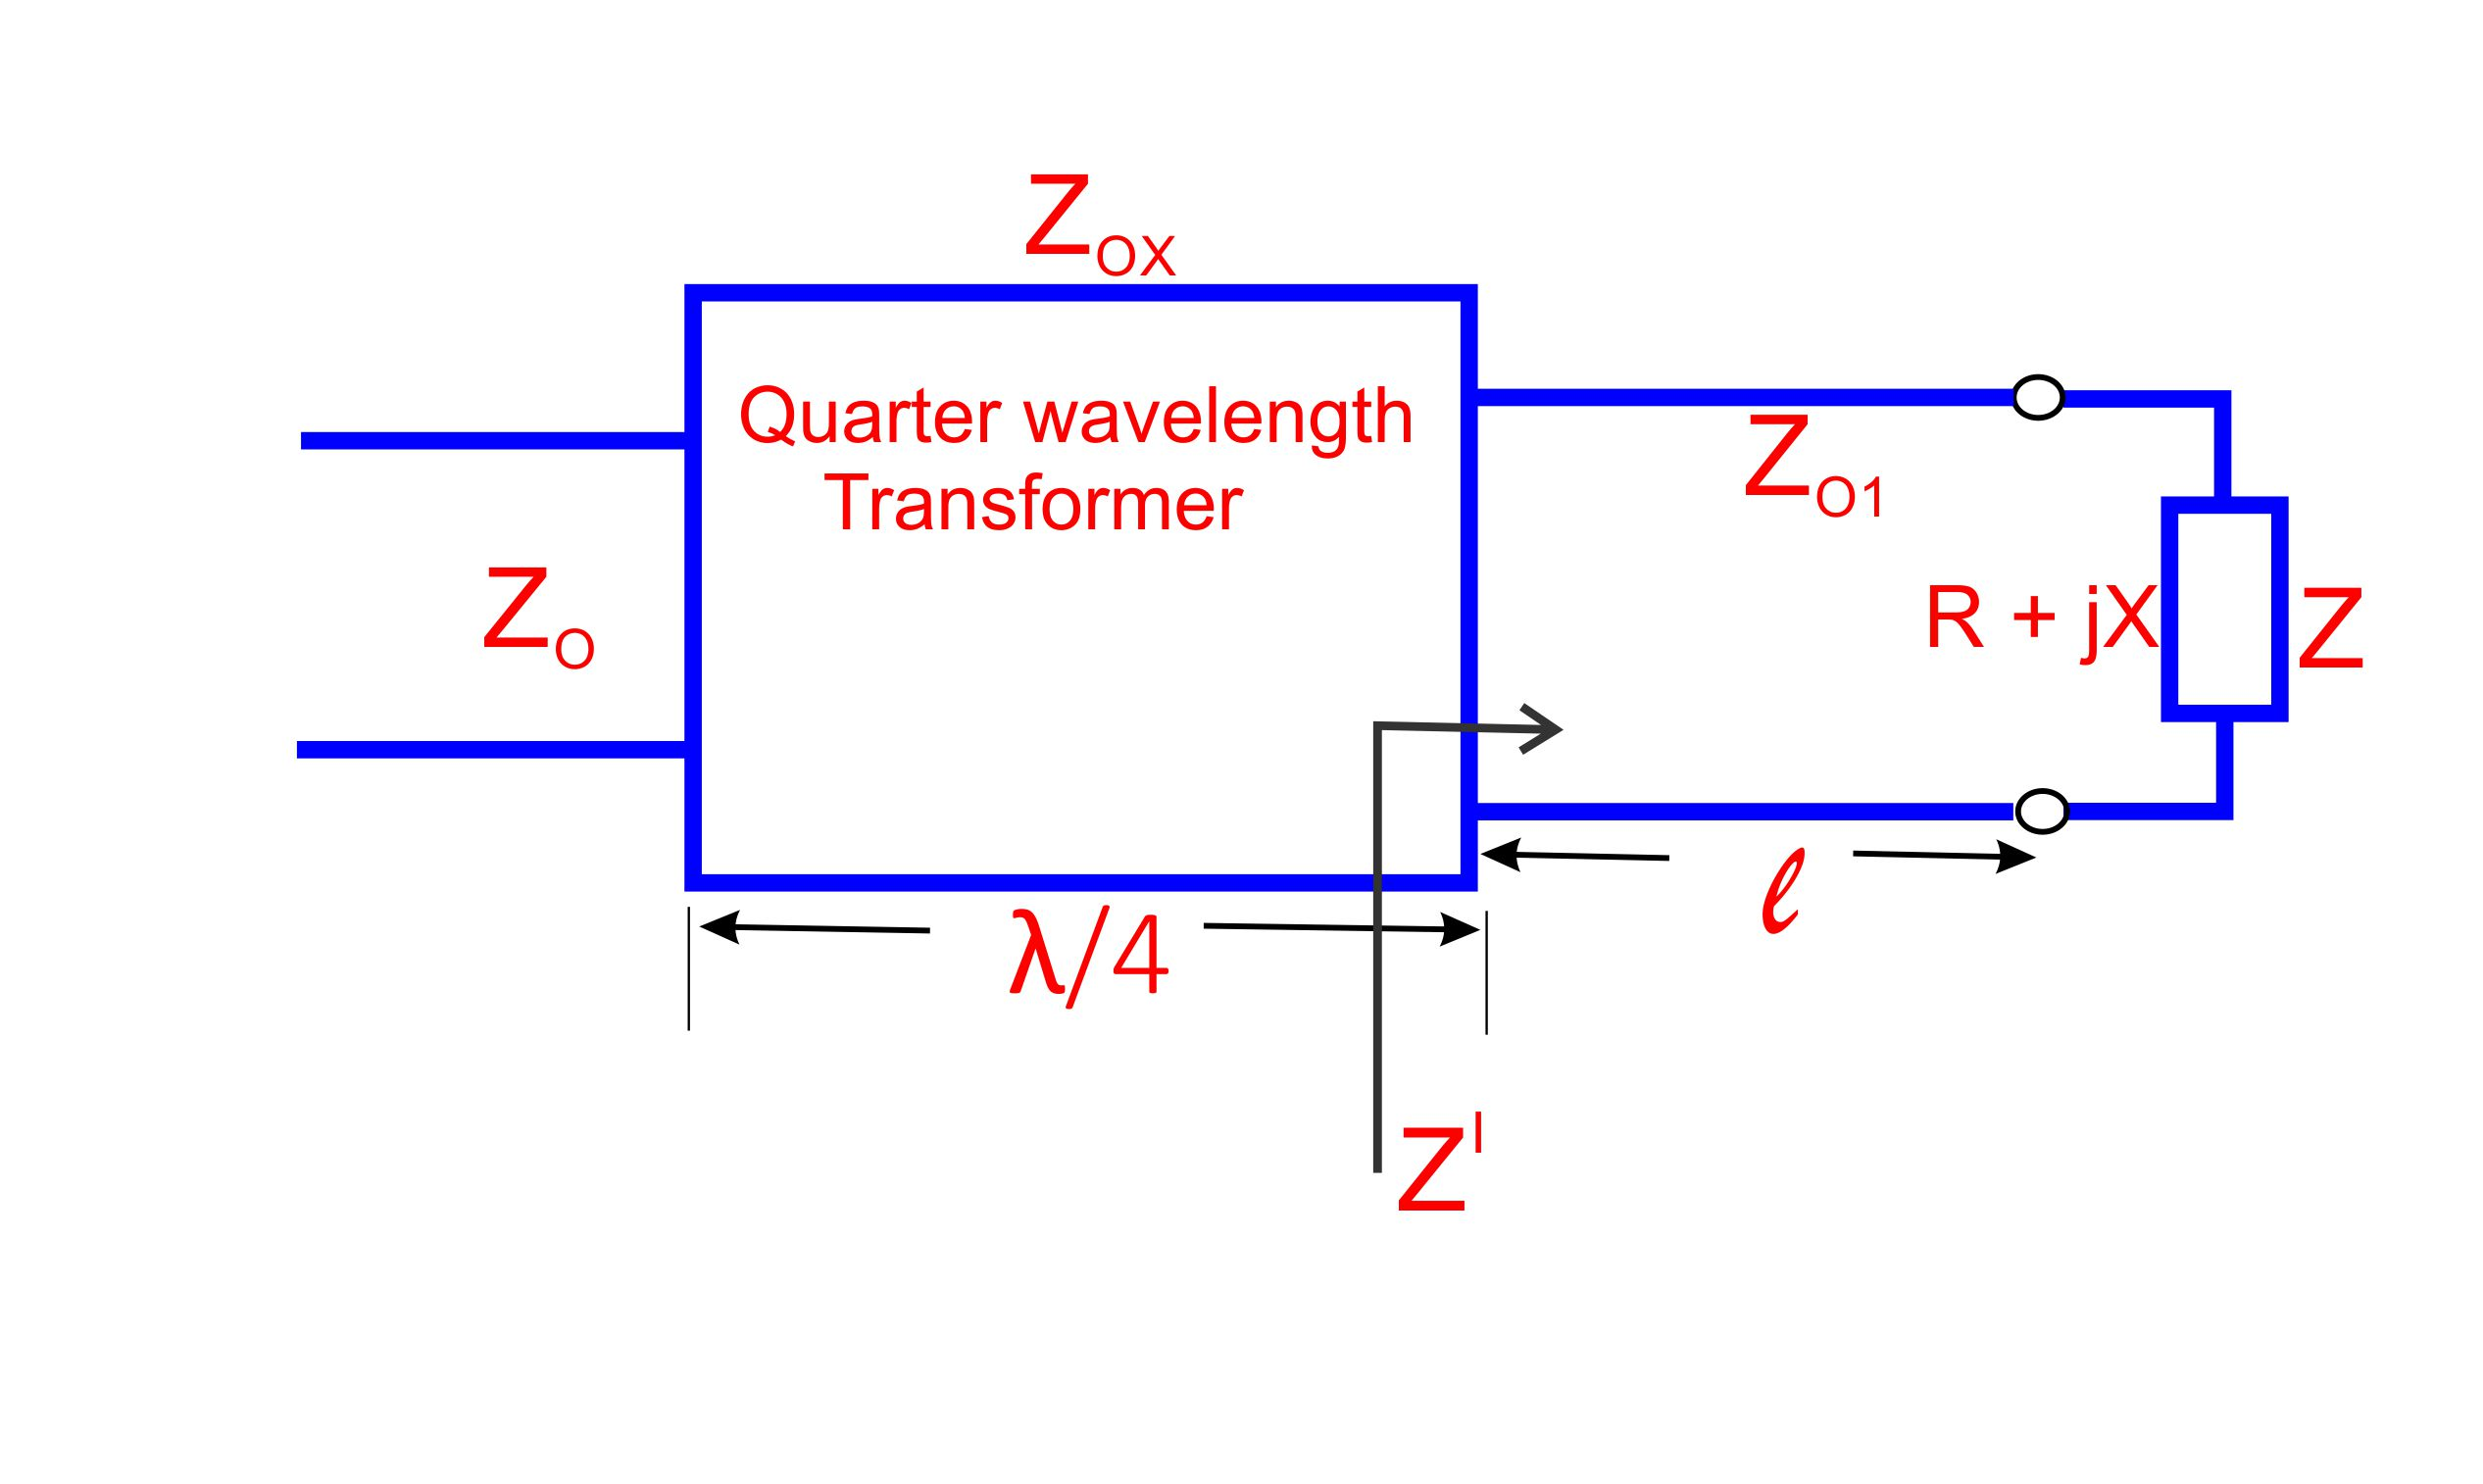
\includegraphics[width=1\linewidth]{\pathtopartone/graphics/fig10}
\caption{The quarter wavelength transformer technique for complex load $Z$}
\label{fig:fig10}
\end{figure}

From figure~\ref{fig:fig10}, we have to move $Z$ which is complex by a distance $l$ on the transmission line to make its transformed impedance real at point B.

\subsubsection*{Procedure:}
\begin{enumerate}[(i)]
\item Mark the normalized point of the impedance, \textbf{P}, $r + jx$\footnote{
The normalized impedance $ \bar{Z}$ is normalized with respect to characteristic impedance of the line $ Z_{01}$, that is $ \bar{Z} = Z/ Z_{01}$
} on the Smith Chart as shown in figure~\ref{fig:sinsmith}.
\begin{figure}[h]
\centering
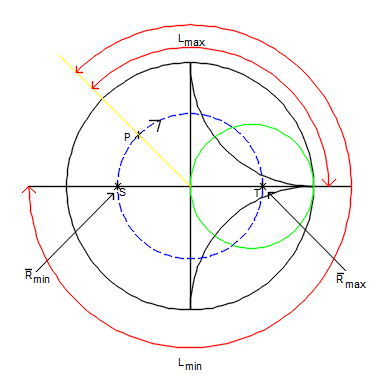
\includegraphics[scale=0.6]{\pathtopartone/graphics/sinsmith}
\caption{ Simplified Smith chart for complex load Quarter wavelength transformer}
\label{fig:sinsmith}
\end{figure}

\item Draw a constant VSWR circle at point \textbf{P} and find the first point of intersection with the real axis moving clockwise. In figure~\ref{fig:sinsmith} it is marked as \textbf{T}. The point \textbf{T} is a real impedance $r_\max$. The next point of intersection with the real axis is \textbf{S} and it is $r_\min$.
\item The respective distances of these points from the load impedance are $ l_\max$ and $ l_\min$ respectively. $ l_\max$ is the distance from point \textbf{P} to \textbf{T}, while $ l_\max$ is the distance from point \textbf{P} to \textbf{S}.
\item Determine the VSWR, $\rho$, and determine the corresponding resistive values $R_\max$ and $R_\min$ at points \textbf{T} and \textbf{S} respectively. 
\item Considering the additional transmission line section of length $ l_\max$, the absolute impedance $ Z'$ seen at point \textbf{T} is
\begin{equation}
Z' = R_\max = Z_{01}\times\rho
\end{equation}
Similarly for $ l_\min$, the absolute impedance $ Z'$ seen at point \textbf{S} is
\begin{equation}
Z' = R_\min = \frac{Z_{01}}{\rho}
\end{equation}
\end{enumerate}
Therefore the absolute impedance $Z'$ at point B in figure~\ref{fig:fig10} can be found using either $ R_\max$ or $ R_\min$ and the characteristics impedance of the quarter wavelength transformer $Z_{0x}$ would be
\begin{equation*}
Z_{0x}=\sqrt{Z_{01}\rho Z_0}\quad\text{or}\quad Z_{0x}=\sqrt{Z_{01}\frac{Z_{01}}{\rho}}
\end{equation*}

Any solution is acceptable depending on whether we want the length $l$ to be small or large. If we are taking cost into consideration, for instance, we will choose a shorter length of the transmission line.

In conclusion, we can say that \textit{Quarter Wavelength Transformer technique} can be used for matching complex impedance $Z$ to the characteristics impedance $Z_0$. However, it has a big drawback in that you require a unique characteristic impedance $Z_{0x}$ for the matching device for different loads. This is not desirable and realizable in nature because, in practice, we do not get a transmission line whose characteristic impedance can be varied easily. The characteristic impedance $Z_{0x}$ depends on the physical dimensions of the transmission line as will be seen in chapter 15. Typically, we have cables of transmission lines with standard characteristic impedance. For example for co-axial cable, the characteristic impedances are $50\Omega$ and $75\Omega$. For parallel wire transmission lines, the characteristic impedances are $300\Omega$ and $600\Omega$.

\begin{exmp}
\subsubsection*{Quarter Wavelength Matching}
A load impedance $Z_{L}=(75-j35)\varOmega$ is to be matched to $50\varOmega$ using a quarter wave transformer. Design the matching set-up. 

\subsection*{Solution}
We recall that the quarter wave transformer can match a resistive load impedance to the characteristic impedance (that is, two resistive impedances). However, the load impedance given is complex, so we use a section of a transmission line of length $l$ as shown in figure~\ref{fig;fighalfwave}, to first convert the impedance to a real value, from that point onward a quarter wave transformer can then be used for the matching.
\begin{figure}[h]
\centering
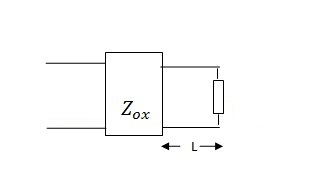
\includegraphics[width=0.7\linewidth]{\pathtopartone/graphics/fighalfwave}
\caption{Load Impedance Matching Design with Quarter Wavelength Trasfromer}
\label{fig;fighalfwave}
\end{figure}

The length of the quarter wave transformer is $\frac{\lambda}{4}$ at XX' (see figure~\ref{fig:image}), $Z_L = (75-j35)\varOmega$ should be real.
\begin{figure}[h]
\centering
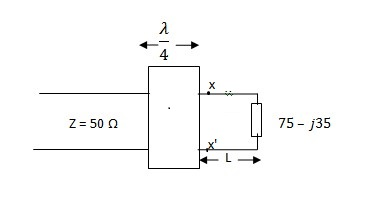
\includegraphics[width=1\linewidth]{\pathtopartone/graphics/image}
\caption{Quarter Wavelength Transformer Design}
\label{fig:image}
\end{figure}

On the Smith chart, we draw the VSWR circle for normalized $Z_{L}$\footnote{
Normalization is done using the characteristic Impedance of the section of the transmission line of length $l$.
} and move clockwise to the point of intersection with the real axis which gives either $R_\min$ or $R_\max$.

Figure~\ref{fig:tosin} shows the Smith chart analysis. $\bar{Z}_L=1.5-j0.7$ is marked at \textbf{X} and the constant VSWR circle is drawn using \textbf{OX} as radius and it intersects the real axis at \textbf{P} and \textbf{Q}. If we move from \textbf{X} to \textbf{P} (\textbf{XP}) we get a resistive impedance corresponding to $r_\min$ and if we move from \textbf{X} through \textbf{P} to \textbf{Q} (\textbf{XPQ}), we get another resistive impedance corresponding to $r_\max$.
\begin{figure}[h]
\centering
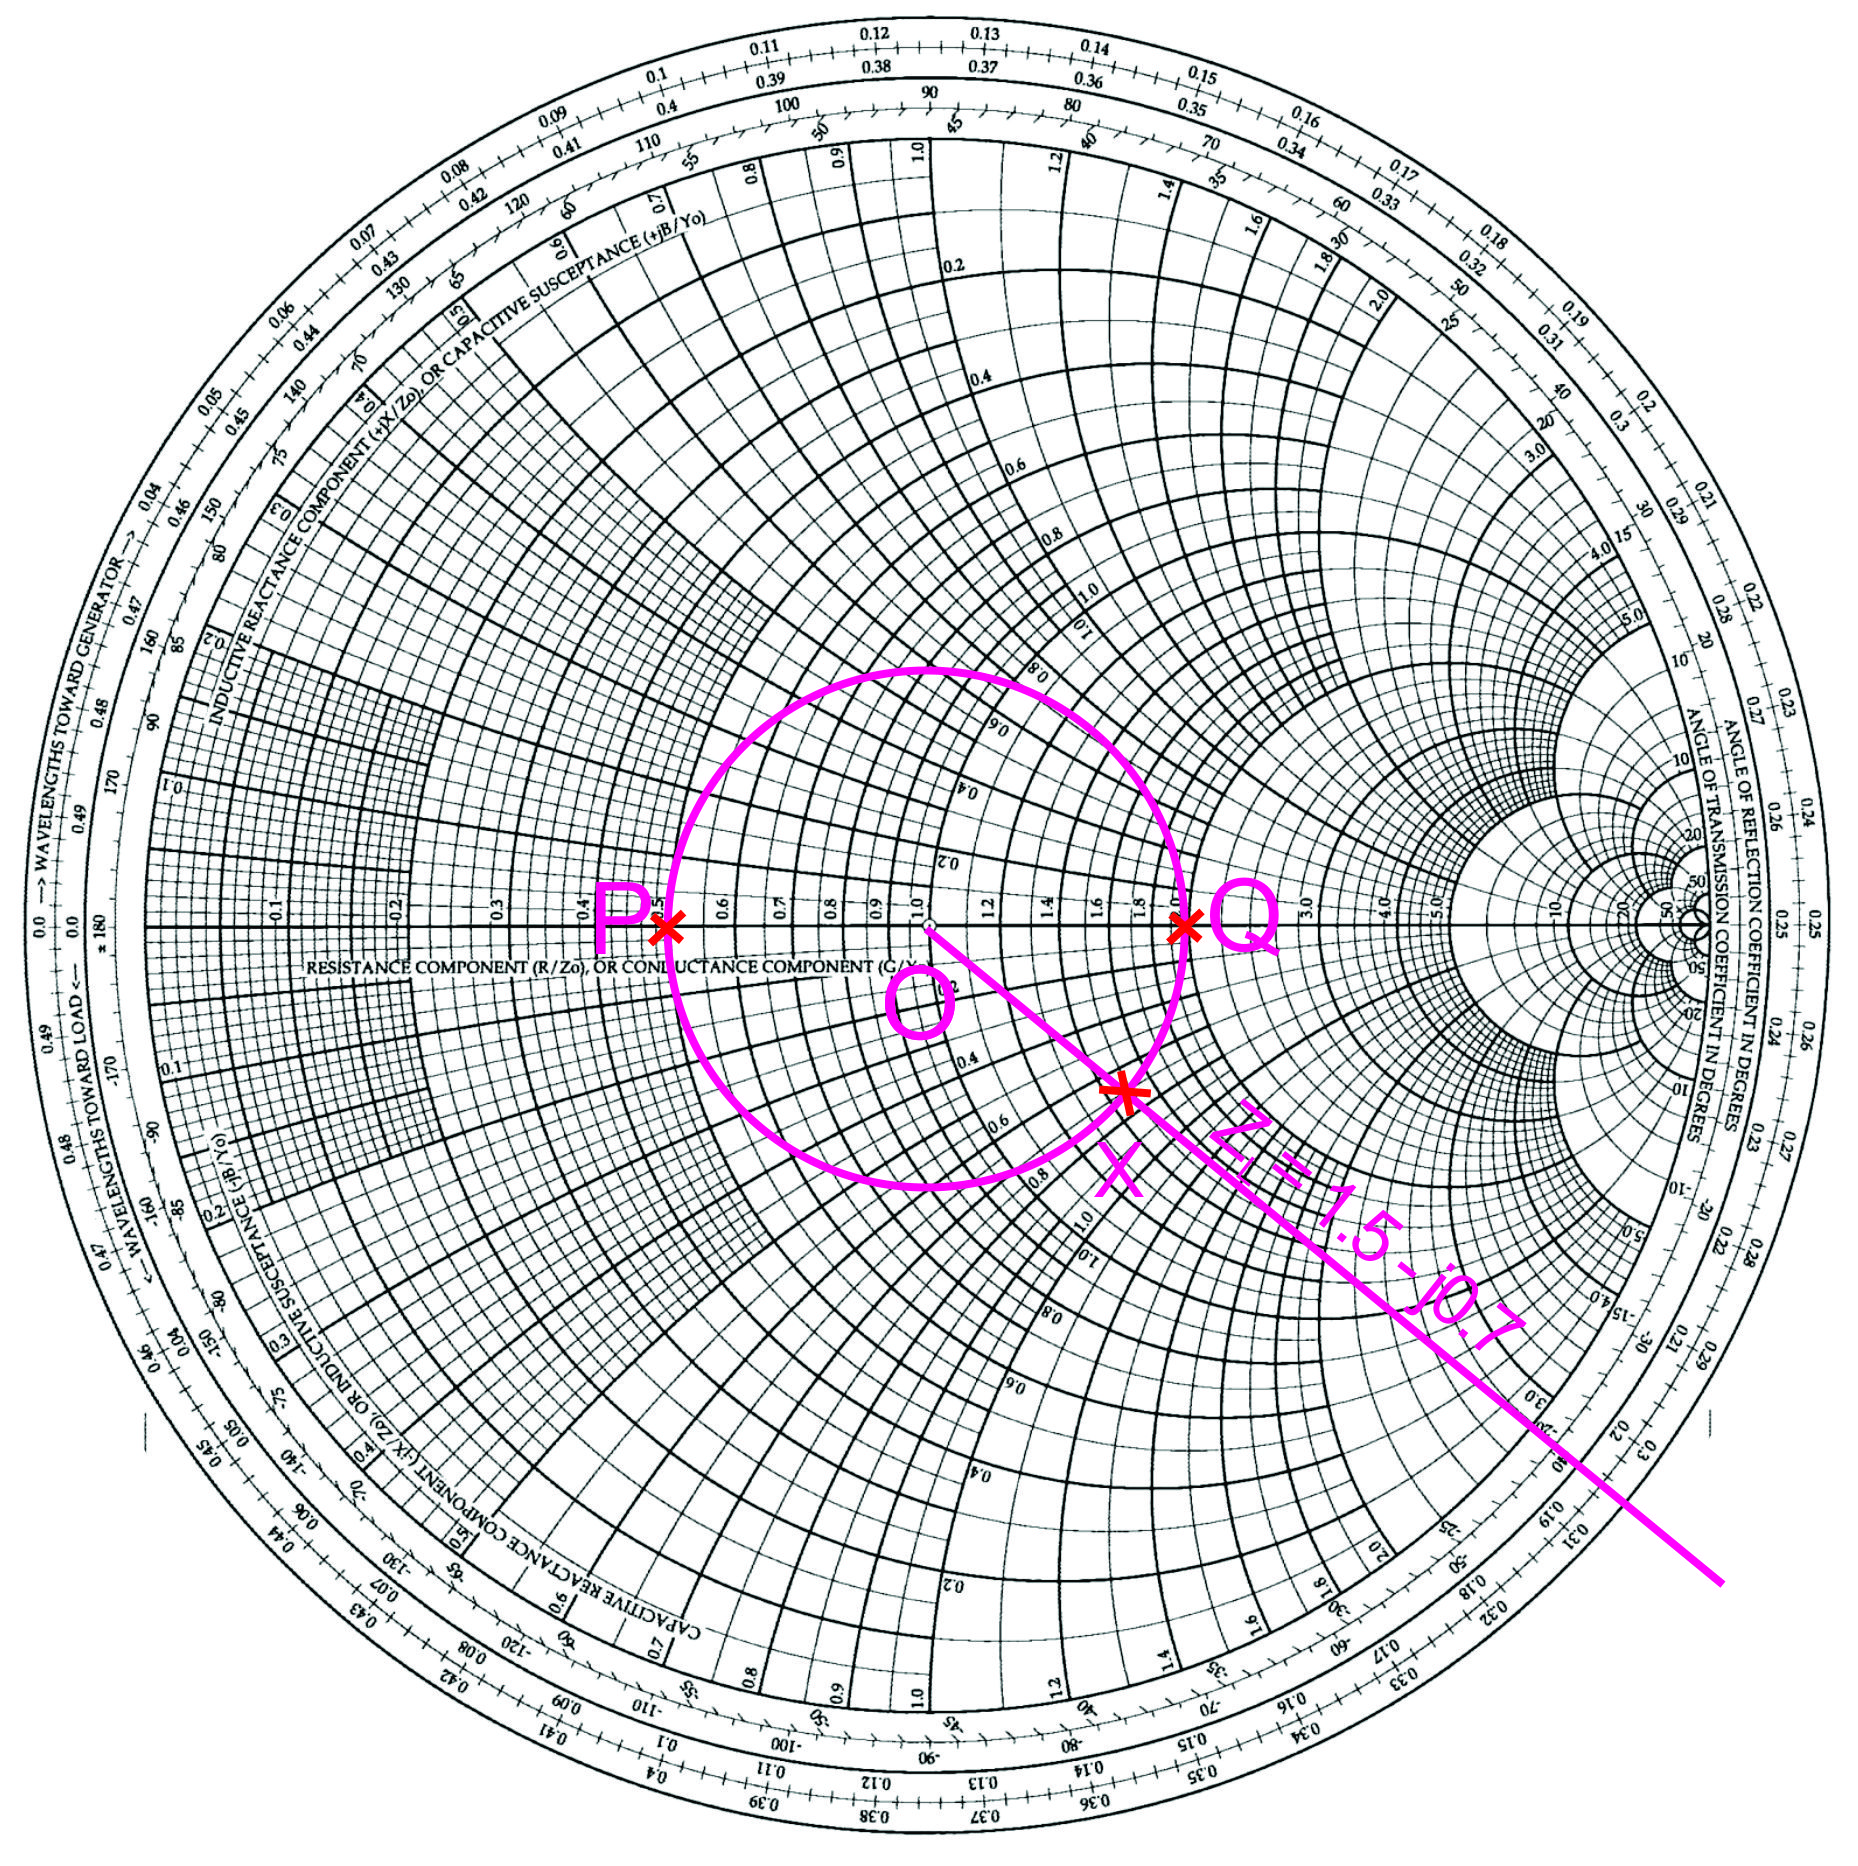
\includegraphics[width=1\linewidth]{\pathtopartone/graphics/TOSIN}
\caption{Quarter Wavelength Design\textemdash\;graphical analysis}
\label{fig:tosin}
\end{figure}

The distance and resistance for \textbf{XP} are
\begin{dmath*}
\boldmath{XP}=0.5\lambda-0.306\lambda
=0.194\lambda
=l_1
\end{dmath*}
\begin{dmath*}
r_\min = \bar{R}_\min \quad\text{From figure~\ref{fig:tosin}}
= 0.5\varOmega
\end{dmath*}

Thus, $R_\min$ is 
\begin{dmath*}
R_\min= Z_0\times\bar{R}_\min
=50\times0.5=25\varOmega
\end{dmath*}

Similarly, the distance and resistance for \textbf{XPQ} are
\begin{dmath*}
\boldmath{XPQ}=0.194\lambda+0.25\lambda
=0.444\lambda
=l_2
\end{dmath*}
\begin{dmath*}
r_\max = \bar{R}_\max\quad\text{From figure~\ref{fig:tosin}}
=2\varOmega
\end{dmath*}

Thus, $R_\max$ is
\begin{dmath*}
R_\max=Z_0 \times \bar{R}_\max
=50\times2
=100\varOmega
\end{dmath*}
Hence $l=l_1=0.194\lambda$ or $l_2=0.444\lambda$ which is the length of the section of the transmission line for transforming the complex impedance to real impedance just before the Quarter Wavelength Transformer.

The outward circle of the Smith chart is calibrated in $\lambda$, so one can take the angle subtended by the movement and do a direct conversion to $\lambda$, $\lambda$\ at X is 0.306 moving to 0.5 is a difference of $0.194\lambda$\footnote{
$l_1=0.5\lambda - 0.306\lambda=0.194\lambda$
}. The top half is $0.25\lambda$, added to the $0.194\lambda$ calculated initially brings us to $0.444\lambda$\footnote{
$l_2=0.25\lambda+0.194\lambda=0.444\lambda$
} for $R_\max$. Going back to the problem we have that for $l_1=0.194\lambda, R_\min=25\varOmega$.
\begin{equation*}
Z_{0x}\footnote{
$Z_{0x}$is the geometric mean of the two impedances to be matched.
} =\sqrt{Z_0 \times R}
=\sqrt{50\times25}
=35.35\varOmega
\end{equation*}
For $l_2=0.444\lambda, R_\max=100\varOmega$ 
\begin{dmath*}
Z_{0x}=\sqrt{Z_0 \times R}
=\sqrt{50\times100}
=70.7\varOmega
\end{dmath*}

Here we see how to match a complex impedance to the characteristic impedance (real impedance) by using a section of the transmission line and the Quarter Wavelength Transformer. The Quarter Wavelength Transformer can match only impedance which is real values, that is why we introduce a section of transmission line before the Quarter Wavelength Transformer to help convert our complex load impedance to real impedance.
\end{exmp}

\subsubsection{Stub Matching Technique}
The question then is, \emph{can we use the standard transmission line which is available with their standardised characteristic impedances?} Yes we can and the approach used is known as \textbf{Stub Matching Technique}\index{stub matching technique}. Let's define a Stub.

\emph{A stub\index{stub} is an auxiliary section of a transmission line which is either short-circuited (S.C) or open-circuited (O.C) that is attached to the main transmission line either in series or parallel.} There are four(4) types of stub matching techniques, which are
\begin{enumerate}[(i)]
\item Series O.C stub matching technique
\item Series S.C stub matching technique
\item parallel O.C stub matching technique
\item Parallel S.C stub matching technique
\end{enumerate}
In this chapter, we are going to be concentrating on the \textbf{Parallel Short Circuit Stub Matching Technique.}

By using the stub at the proper location on the main transmission line, it is possible to match a complex impedance $Z$ to the characteristic impedance $Z_0$.
Recall the advantage of the stub technique is that we do not require a unique characteristic impedance $Z_0$ for each impedance matching. The characteristic impedance of the main and auxiliary transmission lines remains the same. However, we change the length $l_l$ from load to the location of the stub and the length of the stub (or auxiliary transmission line) attached to the main transmission line $l_s$ (see figure~\ref{fig:fig11}).

There are three (3) techniques for matching a stub to the transmission line to match the load impedance to the characteristic impedance and they are:
\begin{enumerate}[(i)]
\item Single Stub matching technique - One attached auxiliary line.
\item Double Stub matching technique - Two attached auxiliary lines.
\item Triple Stub matching technique - Three attached auxiliary lines.
\end{enumerate}

\subsubsection{Single Stub Matching Technique}
In this section, we will discuss the single stub matching technique in the \textit{parallel short circuit stub matching technique configuration}. Figure~\ref{fig:fig11} shows the structure of a single stub matching technique. Again, our aim is to find a real impedance at point A that is equal to the characteristic impedance, $Z_0$. The main transmission line with characteristics impedance $ Z_0$ is connected to load impedance $Z$.
\begin{figure}[h]
\centering
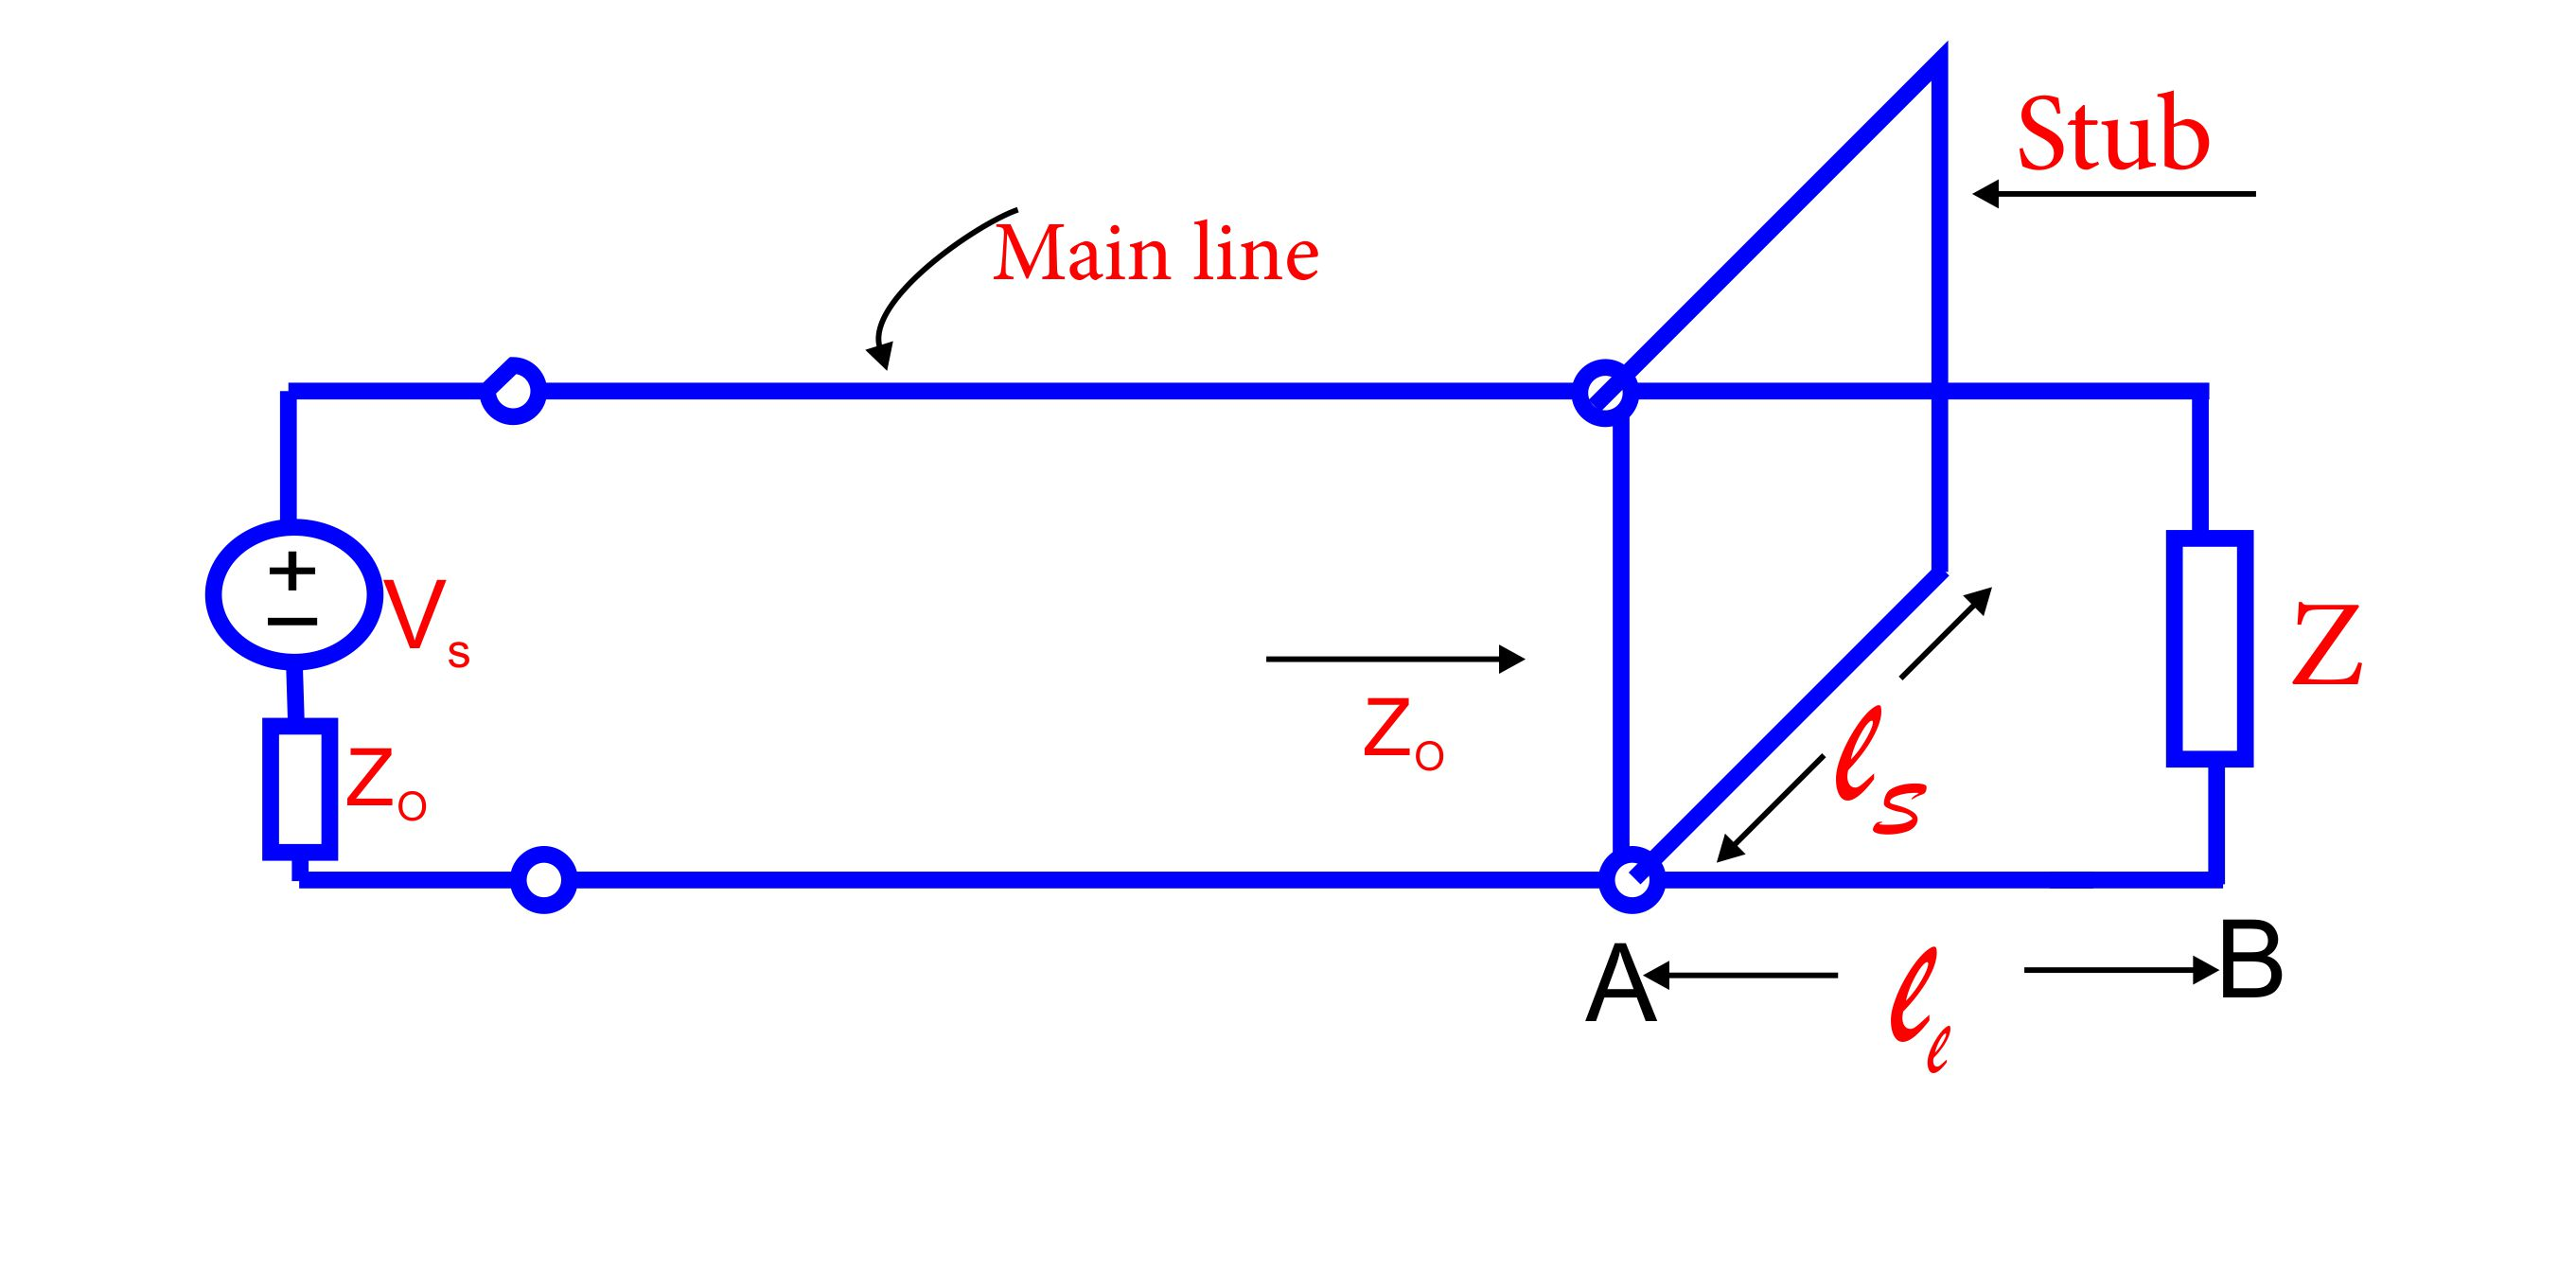
\includegraphics[width=1\linewidth]{\pathtopartone/graphics/fig11}
\caption{Single stub matching technique with one auxiliary transmission line attached}
\label{fig:fig11}
\end{figure}

The stub length $l_s$ is connected in parallel to the main transmission line at a distance $ l_l$ from the impedance to be matched. We know that as voltage or energy moves from the generator to the load, it sees two (2) parts: the stub section and load $Z$ section. At the load, there is a reflection and at the stub, there is a total reflection which is in the opposite direction ($\Gamma_{SC} = -1$) since the stub is short-circuited. If we make sure that both reflected energy from the stub and from the load match each other in amplitude and are opposite in phase, there will be no reflection beyond point A. Since there is no reflection beyond A that is, the input impedance is always going to be equal to the characteristic impedance.

The theory, therefore, is as follows; \emph{we need to find the length $ l_l$ such that when the load impedance $Z$ is transformed by this distance, the resistive part becomes equal to $Z_0$ and the parallel combination of the transformed impedance and the reactive part from the stub cancels out.} We choose $l_s$, such that the reactive part of the stub cancels the reactive part of the load after its transformation. The purpose of the length $l_l$ (location of stub), is to make impedance $Z$ to be equal to characteristic impedance $Z_0$ and the purpose of the length of stub $l_s$ is to neutralize the reactive part. We will proceed to solve the single stub matching technique graphically using the Smith Chart.

For the single stub matching, we will work in terms of admittance since we have parallel connections. Therefore, let the load admittance and characteristic admittance be
\begin{align*}
Y &= 1/Z\quad\text{(load admittance)}\\
Y_0 &= 1/Z_0\quad\text{(characteristic admittance)}
\end{align*}
Hence, the normalized load admittance is
\begin{equation*} 
\bar{Y}=\frac{Y}{Y_0} 
\end{equation*}
Figure~\ref{fig:qwtch} shows the simplified Smith Chart for the single stub matching problem.
\begin{figure}[h]
\centering
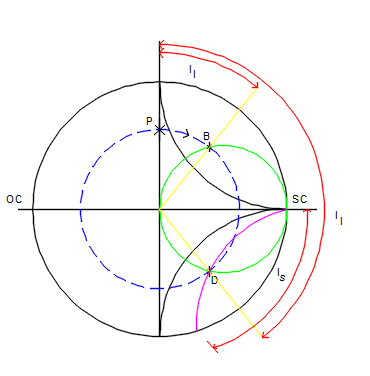
\includegraphics[width=1\linewidth]{\pathtopartone/graphics/qwtch}
\caption{Simplified Smith Chart for Single Stub Matching}
\label{fig:qwtch}
\end{figure}
Let P be the point of the normalized admittance to be matched and the dashed circle passing through P is the constant VSWR circle. Where this circle intersects $g = 1$ circle denoted by points B and D, we have that the real part of the transformed admittance, $Y$ equals the characteristic admittance $Y_0$. That is, at points B and D, the distance from P to B or P to D will give us a conductive part equal to unity (same as $Y_0$) and then what the unmatched reactive part should be at those locations. These locations give the value of $l_l$ which corresponds to point A in figure~\ref{fig:fig11}, such that from the load section, $\bar{Y} = 1 + jb'$. Therefore, the stub must have $-jb'$ as its admittance so that when they are connected in parallel, the susceptance cancels out leaving only the normalised admittance of $1 + j0$. The process involved is summarized as follows:
\begin{enumerate}[(i)]
\item First locate the given admittance value to be matched on the Smith Chart.
\item Draw your constant VSWR circle through the located point on Smith Chart.
\item Move along the constant VSWR circle in a clockwise direction and mark the two points it intersects with the constant $g = 1$ circle.
\item The distance from the first location (point P) to either of these new points (point B or D) is the location of stub $l_l$.
\item Choose a point from the new points say point B (1+j$b'$), and take a mirror image which is point D (1 - j$b'$). Draw a constant susceptance circle passing through this point D. Where this circle touches the outermost circle of the Smith Chart is $-jb'$.
\item The distance moving anticlockwise from this point S to the SC point on the Smith Chart gives us the length of the stub (see figure~\ref{fig:qwtch}).
\end{enumerate}

Similarly, when the stub is connected in series, we use the same pattern but we will use impedance values instead of admittances. The single stub matching technique is extremely useful in matching impedances to the characteristic impedance of the line. In this technique, we are matching impedance without any unique transmission line unit as in the case of a Quarter Wavelength Transformer Technique. However, this technique has a small drawback which is that the location of the stub depends on the impedance to be matched. Though the single stub technique can match all possible loads, for every load to be matched, the location of the stub has to be changed which may not be that easy once the stub is connected. To solve these limitations as we did for quarter wavelength transformer technology, we will use the Double Stub Matching Technique.

\begin{exmp}
\subsubsection*{Single Stub Matching}
Design a single stub matching unit to match the load impedance shown in figure~\ref{fig:figw} to the characteristic impedance, $Z_0 = 50\varOmega$. Calculate for $l_s$ and $l_1$.
\begin{figure}[h]
\centering
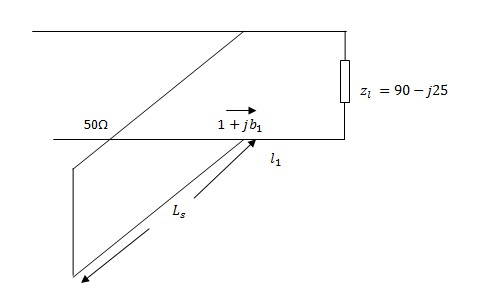
\includegraphics[width=1\linewidth]{\pathtopartone/graphics/figw}
\caption{Single Stub Matching design}
\label{fig:figw}
\end{figure}

\subsection*{Solution}
We normalize $Z_L=90-j25$ to get 
$\bar{Z}_L=1.8-j0.5$. since stub and $Z_L$ are in parallel,
we convert $\bar{Z}_L$ to its admittance value. $\bar{Y}_{L}$
should be transformed from 
$\bar{Y}_{L}$=$g+jb$ to $1+jb_1$ hence it lies on the circle of constant conductance $g=1$. With OP we draw a circle of constant VSWR with OP as radius. We get the point where this VSWR circle intercept the g=1 circle at moving clockwise(towards the generator )from Q to M. The distance QM correspond to $L_1, L_1=0.152\lambda-0.032\lambda=0.12\lambda$.

Mirror M on the VSWR circle to get $1-jb1$. On the constant susceptance curve of $jb$, find where it intercepts the circle at $g=0 \ and \ ?jb_1$. This is the outermost circle. $R$ represent the pure susceptance value of $jb_1$. 
\begin{figure}[h]
\centering
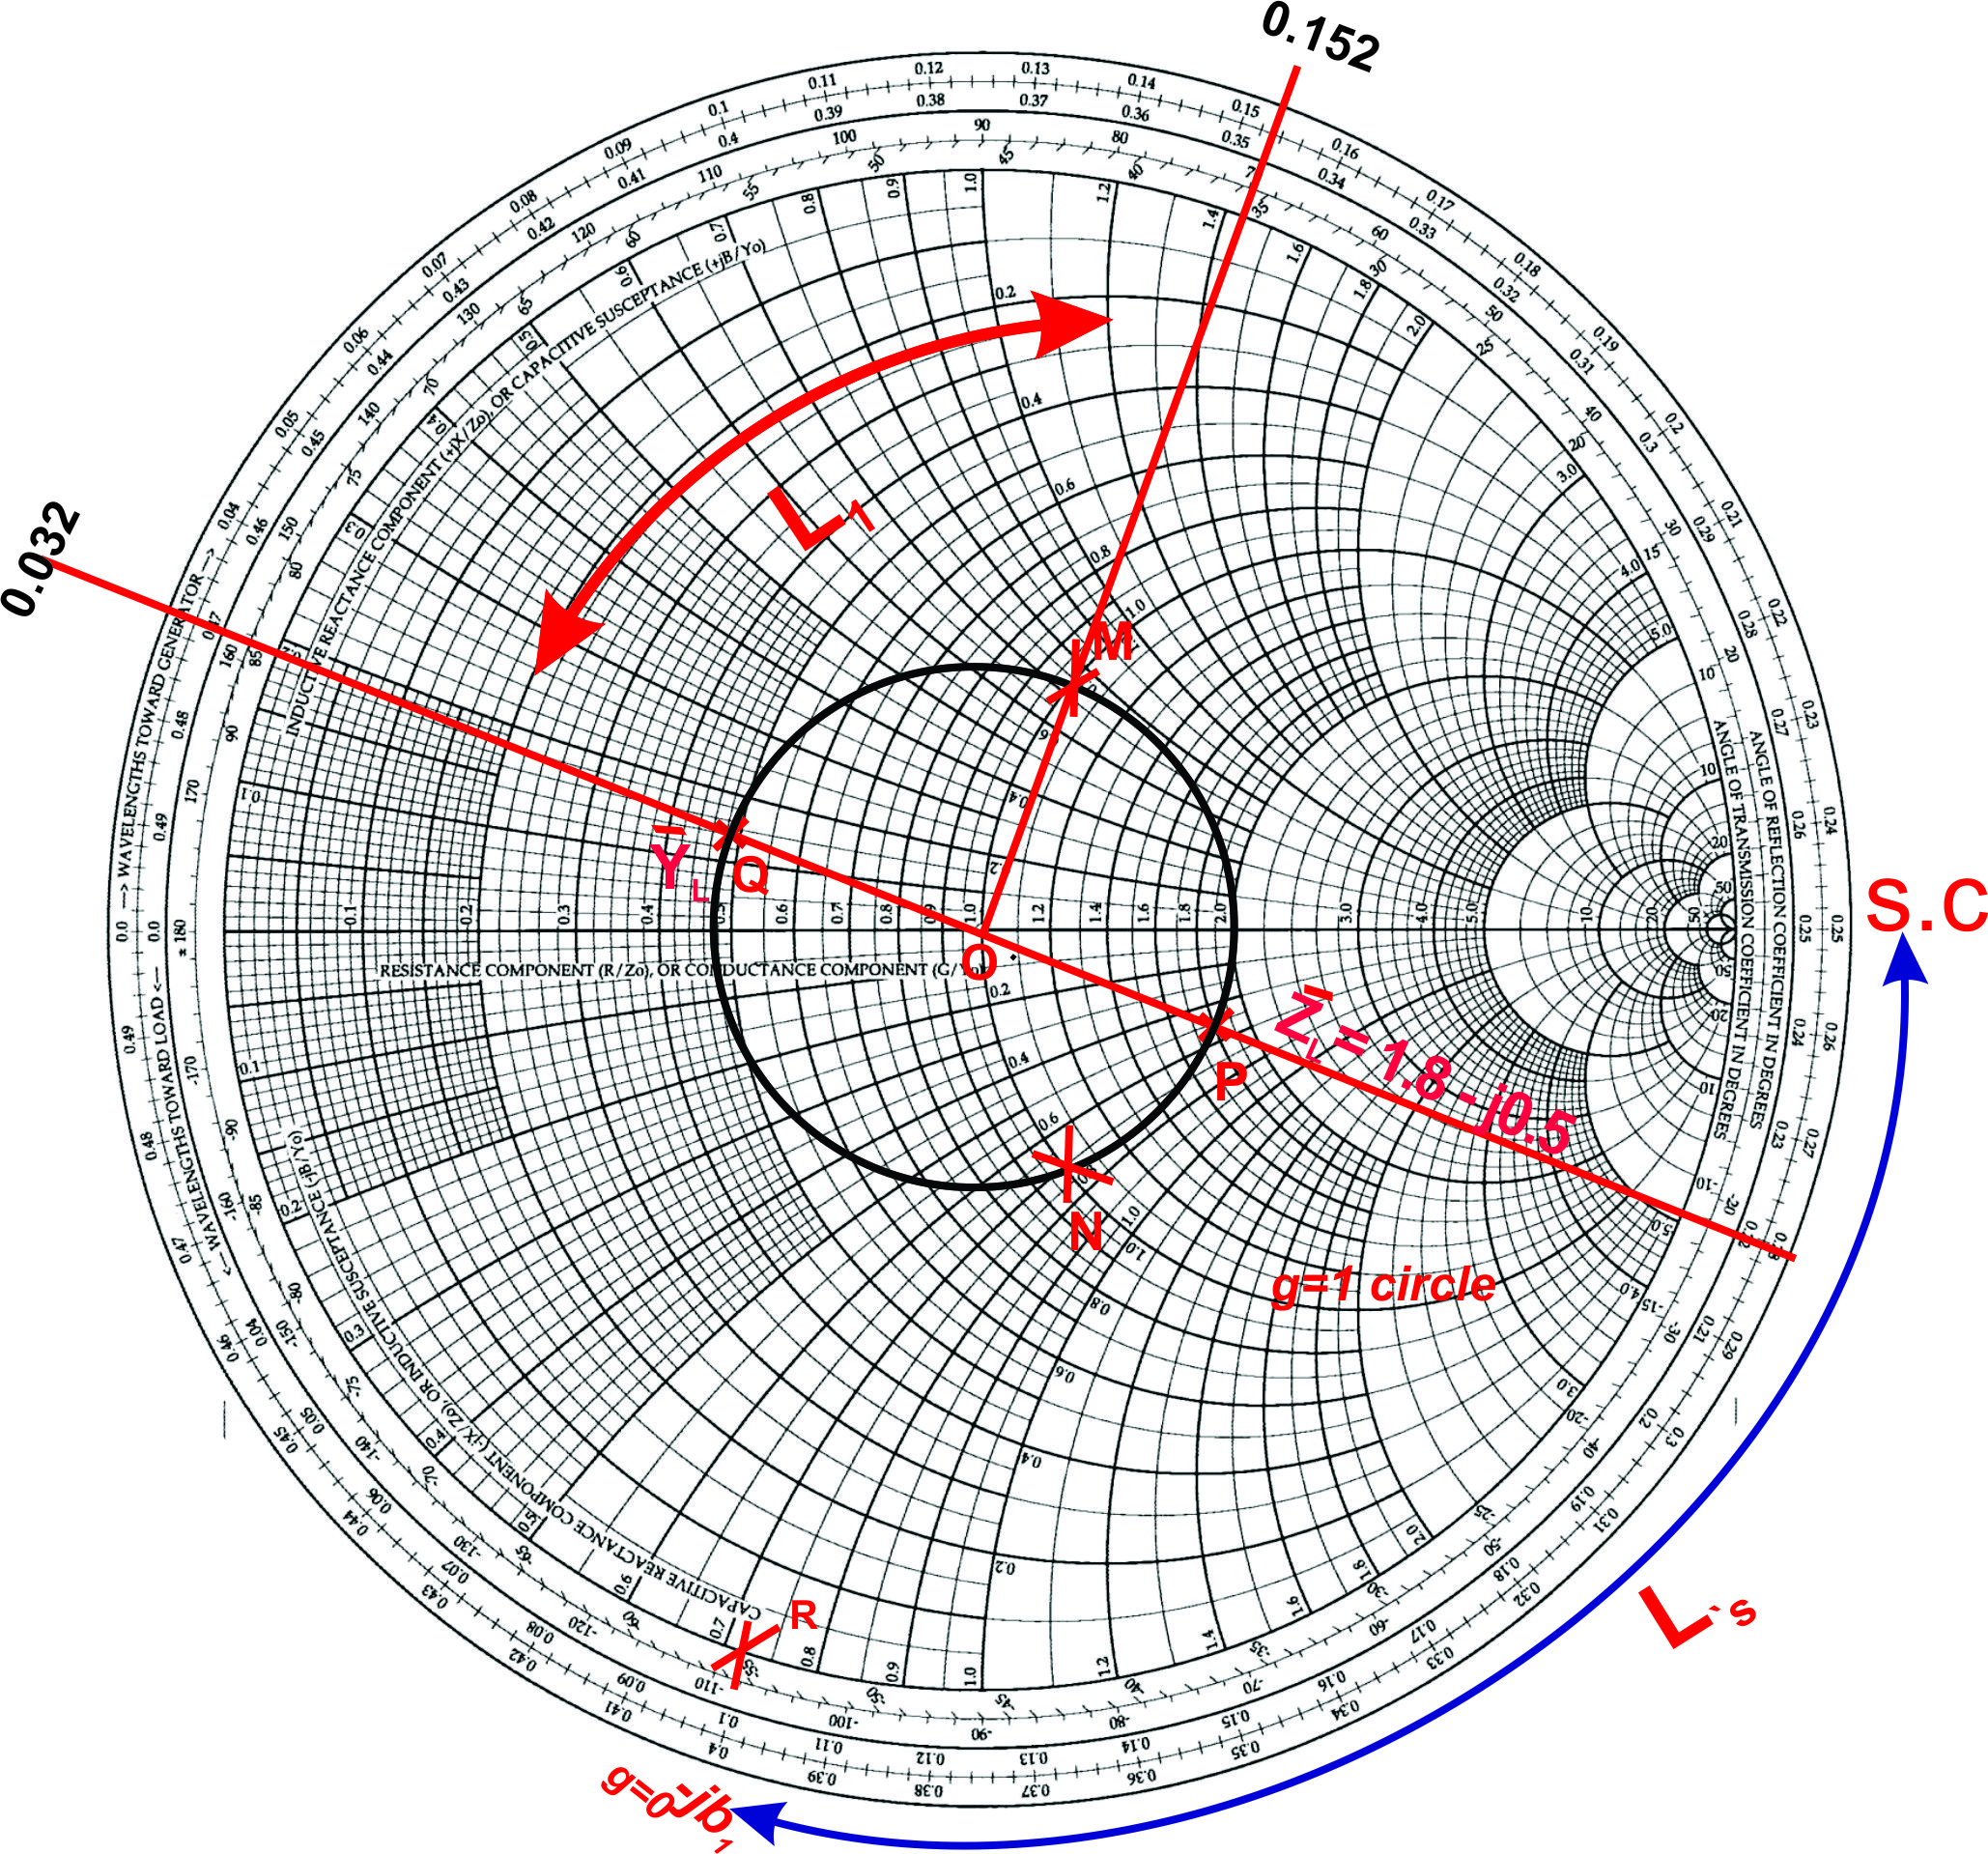
\includegraphics[width=1\linewidth]{\pathtopartone/graphics/fig14}
\caption{Single Stub Matching Design\textemdash\;graphical analysis}
\label{fig:fig14}
\end{figure}

Hence we have to move from the short circuit (SC) end of the stub towards the generator to see this Susceptance. The distance $l_s$ is the movement from SC to -jb1 towards the generator and that distance represents the length of the stub. For admittance on the Smith chart right most side is the SC part and the leftmost part is the open circuit part. This is opposite to the convention in the impedance Smith chart.

At SC $l_{sc}=0.25\lambda$ moving towards the generator.At R, $l=0.402\lambda$,the distance $l_s=0.402-0.25=0.152\lambda$. Now we know the length of the stub and the location of the stub as well. These are some of the problems which can be solved easily with the help of the Smith chart. Using an analytic approach for the same process is an extremely tedious task. This example clearly demonstrates the use of a Smith chart for solving complex transmission line problems.
\end{exmp}

\subsubsection{Double Stub Matching Technique}\index{double stub matching technique}
This technique involves the use of two (2) stubs. In this method, we change only the length of the stub while the location of the stub is fixed. The separation between the stubs is $3\frac{\lambda}{8}$. The distance between stub 1 and load is $l_l$ as shown in figure~\ref{fig:fig12}
%put footnote here and two figures(double stub(12.9) and Smith Chart(12.10))%
\begin{figure}[h]
\centering
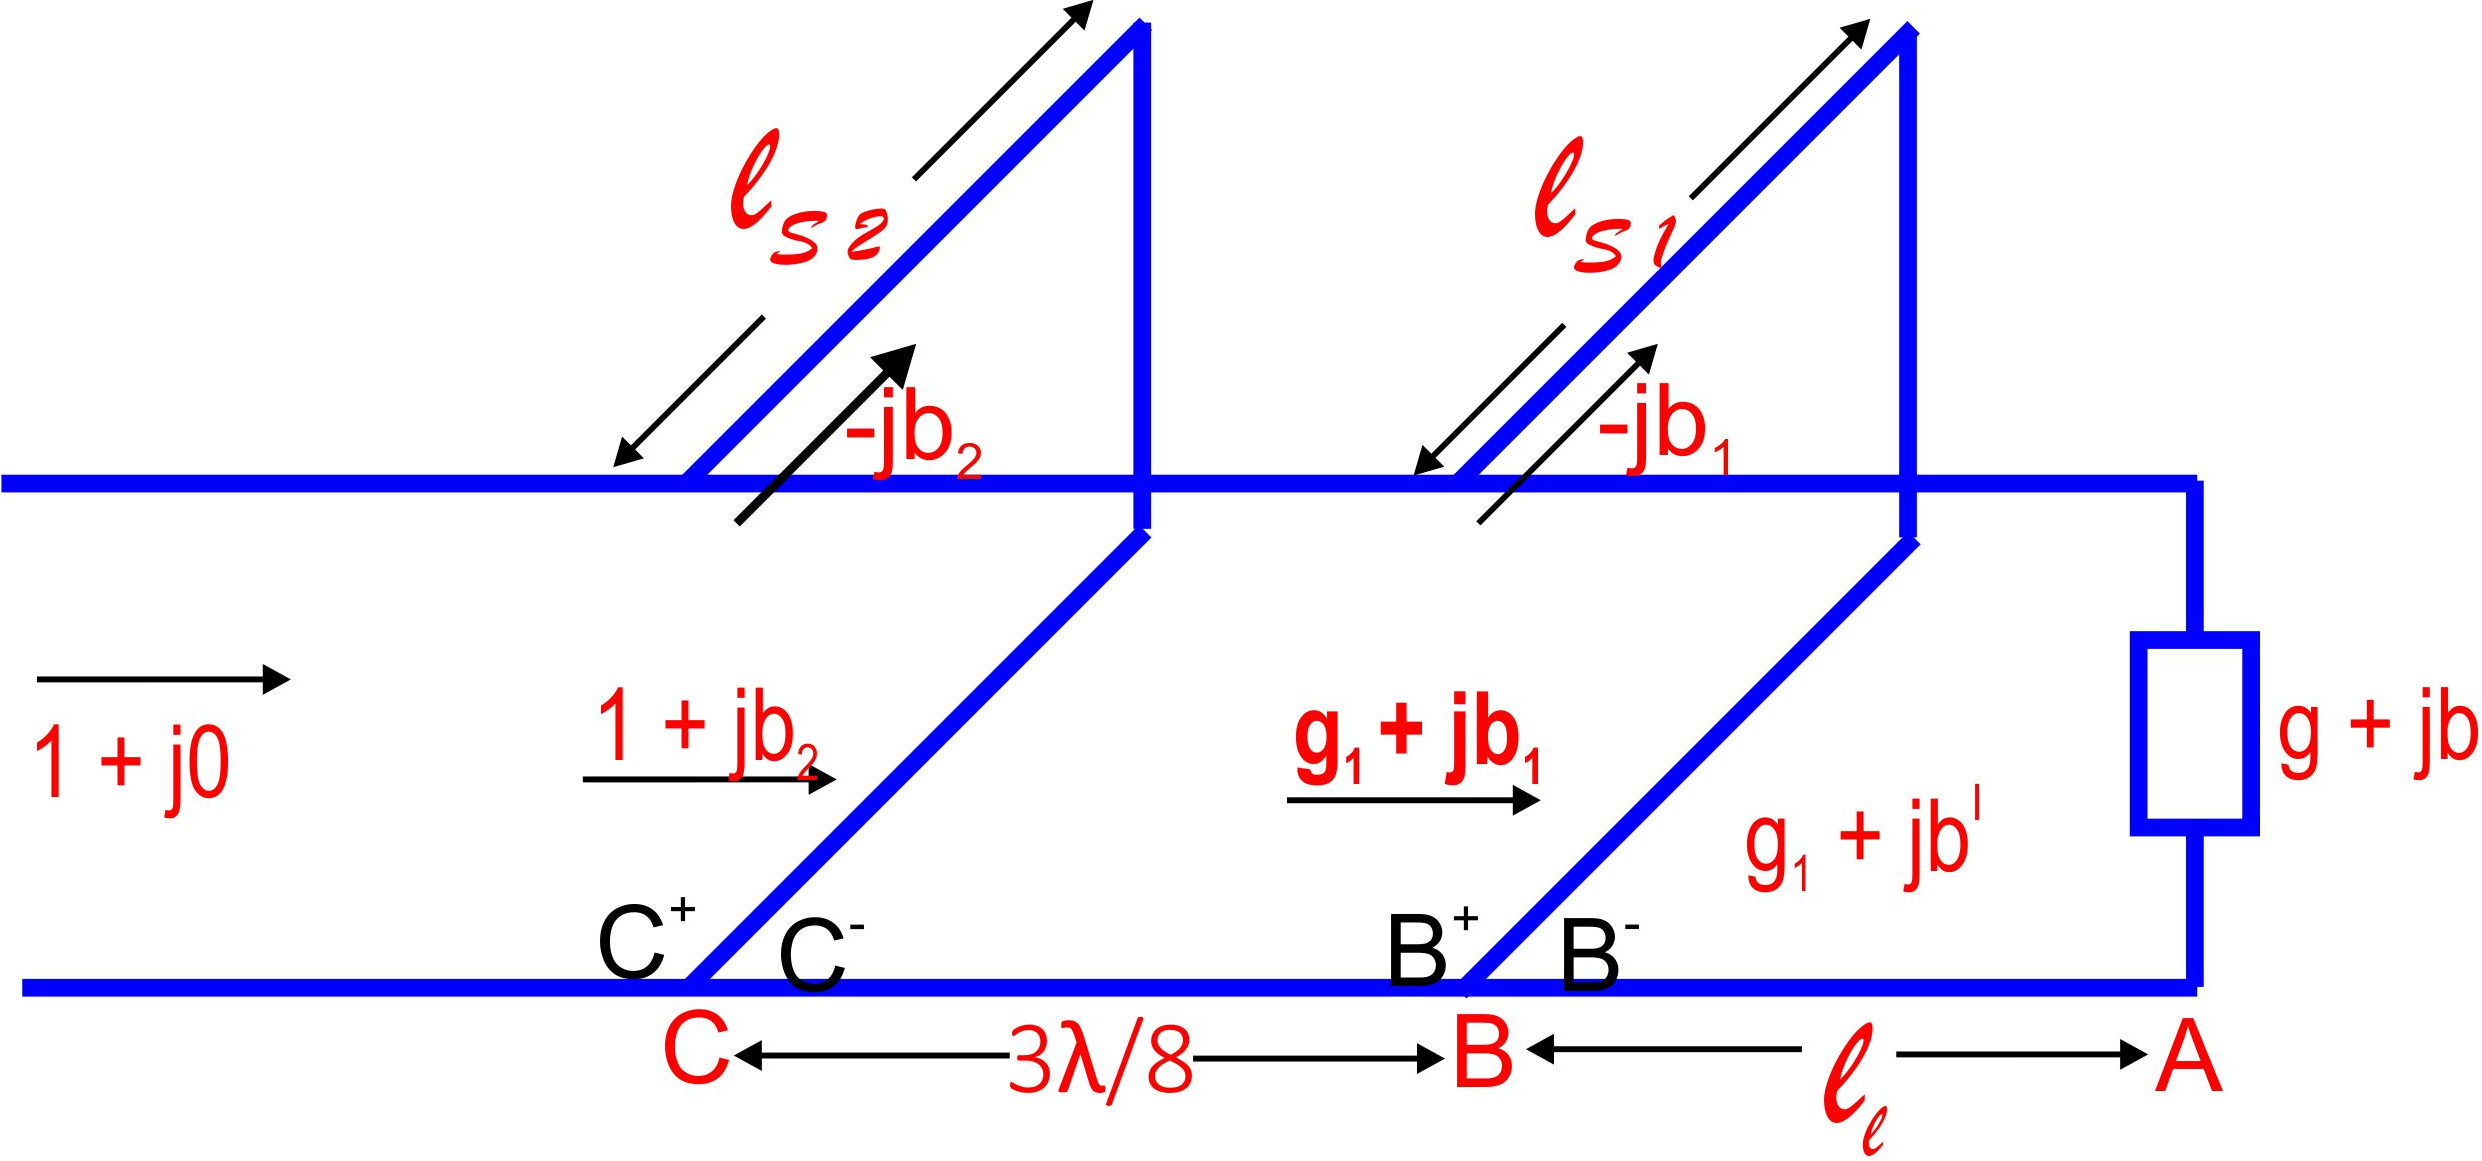
\includegraphics[width=1\linewidth]{\pathtopartone/graphics/fig12}
\caption{Double Stub Matching Technique with two auxiliary lines attached}
\label{fig:fig12}
\end{figure}
From figure~\ref{fig:fig12}, starting from the load end, the initial admittance is $\bar{Y} = g + jb$. After a distance $l_l$ moving clockwise to point B (towards generator), (at this point B\textsuperscript{\textemdash}, $g_1 + jb'$) and when this is combined with the susceptance from stub 1, $-jb_1$, we get $g_1 +jb_1$ at B\textsuperscript{+}. When transformed along the length $3\frac{\lambda}{8}$, we get $1 + jb_2$. When this is combined with the susceptance of stub 2 $-jb_2$, we get $1 + 0j$ beyond point C, C\textsuperscript{+}. As for the single-stub matching technique, we will solve the double-stub matching technique using the Smith Chart.
\begin{figure}[h]
\centering
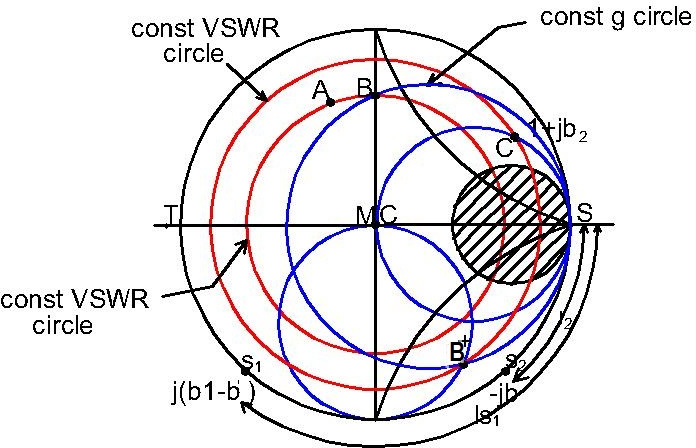
\includegraphics[width=1\linewidth]{\pathtopartone/graphics/dousmith}
\caption{Simplified Smith Chart for Double Stub Matching Technique}
\label{fig:dousmith}
\end{figure}

Figure~\ref{fig:dousmith} shows the analysis for the structure in figure~\ref{fig:fig12}. We have already seen in the single stub matching technique that at the location where a stub is connected if the admittance seen towards the load is of the form $1 +jb$ then the stub can cancel the reactive part of the admittance and we get a matching condition. In the case of the double stub matching technique, if the admittance at point C is of the form $1 + jb$, the matching condition can be achieved. This means at location B the admittance must be a transformed version of $1 + jb$ by a distance $3\frac{\lambda}{8}$ away from the generator. The translation of $1 + jb$ by a distance of $3\frac{\lambda}{8}$ counter-clockwise is the same as the rotation of the $g = 1$ circle by 270\textdegree counter-clockwise around the centre of the Smith Chart.

\subsubsection*{Procedure:}
\begin{enumerate}[(i)]
\item Mark the normalized admittance $g + jb$ denoted by A in figure~\ref{fig:dousmith}.
\item Move on the constant VSWR circle by $l_l$ to get to point B\textsuperscript{\textemdash} ($g_1 + jb'$).
\item At point B\textsuperscript{+}, since we are adding the admittance of stub 1, $-jb'$, we are changing only the reactive part. So we move anticlockwise on the circle of constant conductance, $g_1$, from B\textsuperscript{\textemdash} till we get to the rotated $g = 1$ circle where it intersects at B\textsuperscript{+}. Essentially, stub 1 helps in bringing the admittance to lie on the rotated circle.
\item At point B\textsuperscript{+}, we now move on a constant VSWR circle in a clockwise direction by $ 3\frac{\lambda}{8}$ to transform the admittance $g_1 + jb_1$ to $1 + jb_2$ at C\textsuperscript{\textemdash}.
\item To cancel the reactive part, $jb_2$ we take a mirror image, $1-jb_2$, then find susceptance circle of $-jb_2$ at the outermost circle of the Smith Chart, $S_2$. We measure the distance from this point to the SC point in an anticlockwise direction to give us the length of the second stub, $l_{s2}$.
\item Now to find the length of the first stub, we find the difference between the two (2) susceptance values B\textsuperscript{\textemdash} and B\textsuperscript{+} since the conductance is the same. Mark the difference on the outermost circle of the Smith Chart $S_1$. The distance from this point to the SC point moving anticlockwise gives the length of the first stub.
\end{enumerate}

We have successfully tackled the drawback of the flexible location of the stub in the single stub matching technique. However, the double stub matching technique has a drawback which is, the whole essence of matching is possible provided that by moving in a constant conductance circle we can intersect the $g = 1$ circle. If by the movement through the constant conductance circle, we can not reach the rotated $g = 1$ circle, then matching is not possible. Now we know the nature of the constant g circle (that they are within one another), so it is possible that if the admittance at point B\textsuperscript{\textemdash} lies in a circle smaller than the $g = 1$ circle, then by our movement inside the constant conductance circle, we will never be able to intersect the rotated $g = 1$ circle, which means matching is not possible. What this means is that if $g_1 + jb'$ lies within the shaded forbidden region shown in figure~\ref{fig:dousmith}, then impedance matching is not possible. The impedance we want to match can lie in the forbidden region, but the transformed impedance after distance $ l_l$ should be out of the forbidden region.

So by choosing a proper value for $l_l$, we can avoid the forbidden region. Therefore, the double stub matching technique has a small limitation that it cannot match those impedances whose transformed value after $l_l$ lies within the forbidden region. However, this has been solved by introducing the concept of \emph{three stub matching}\index{three stub matching}.

\begin{exmp}
\subsubsection*{Double stub matching technique}
For a load impedance, $Z_{L} = (100 + j100)\Omega$, and characteristic impedance, $Z_0 = 50\Omega$,  design a double stub matching unit to match the load for the transmission line. Note $l_{1} = 0.4\lambda$.

\subsubsection*{Solution}			
\subsubsection*{Procedure:}
\begin{enumerate}[(i)]
\item Determine the normalized value for the load resistance $Z_{L}$.
\begin{dmath*}
\bar{Z_{L}} = \frac{Z_{L}}{Z_0} = 2 + j2
\end{dmath*}
\begin{figure}[h]
\centering
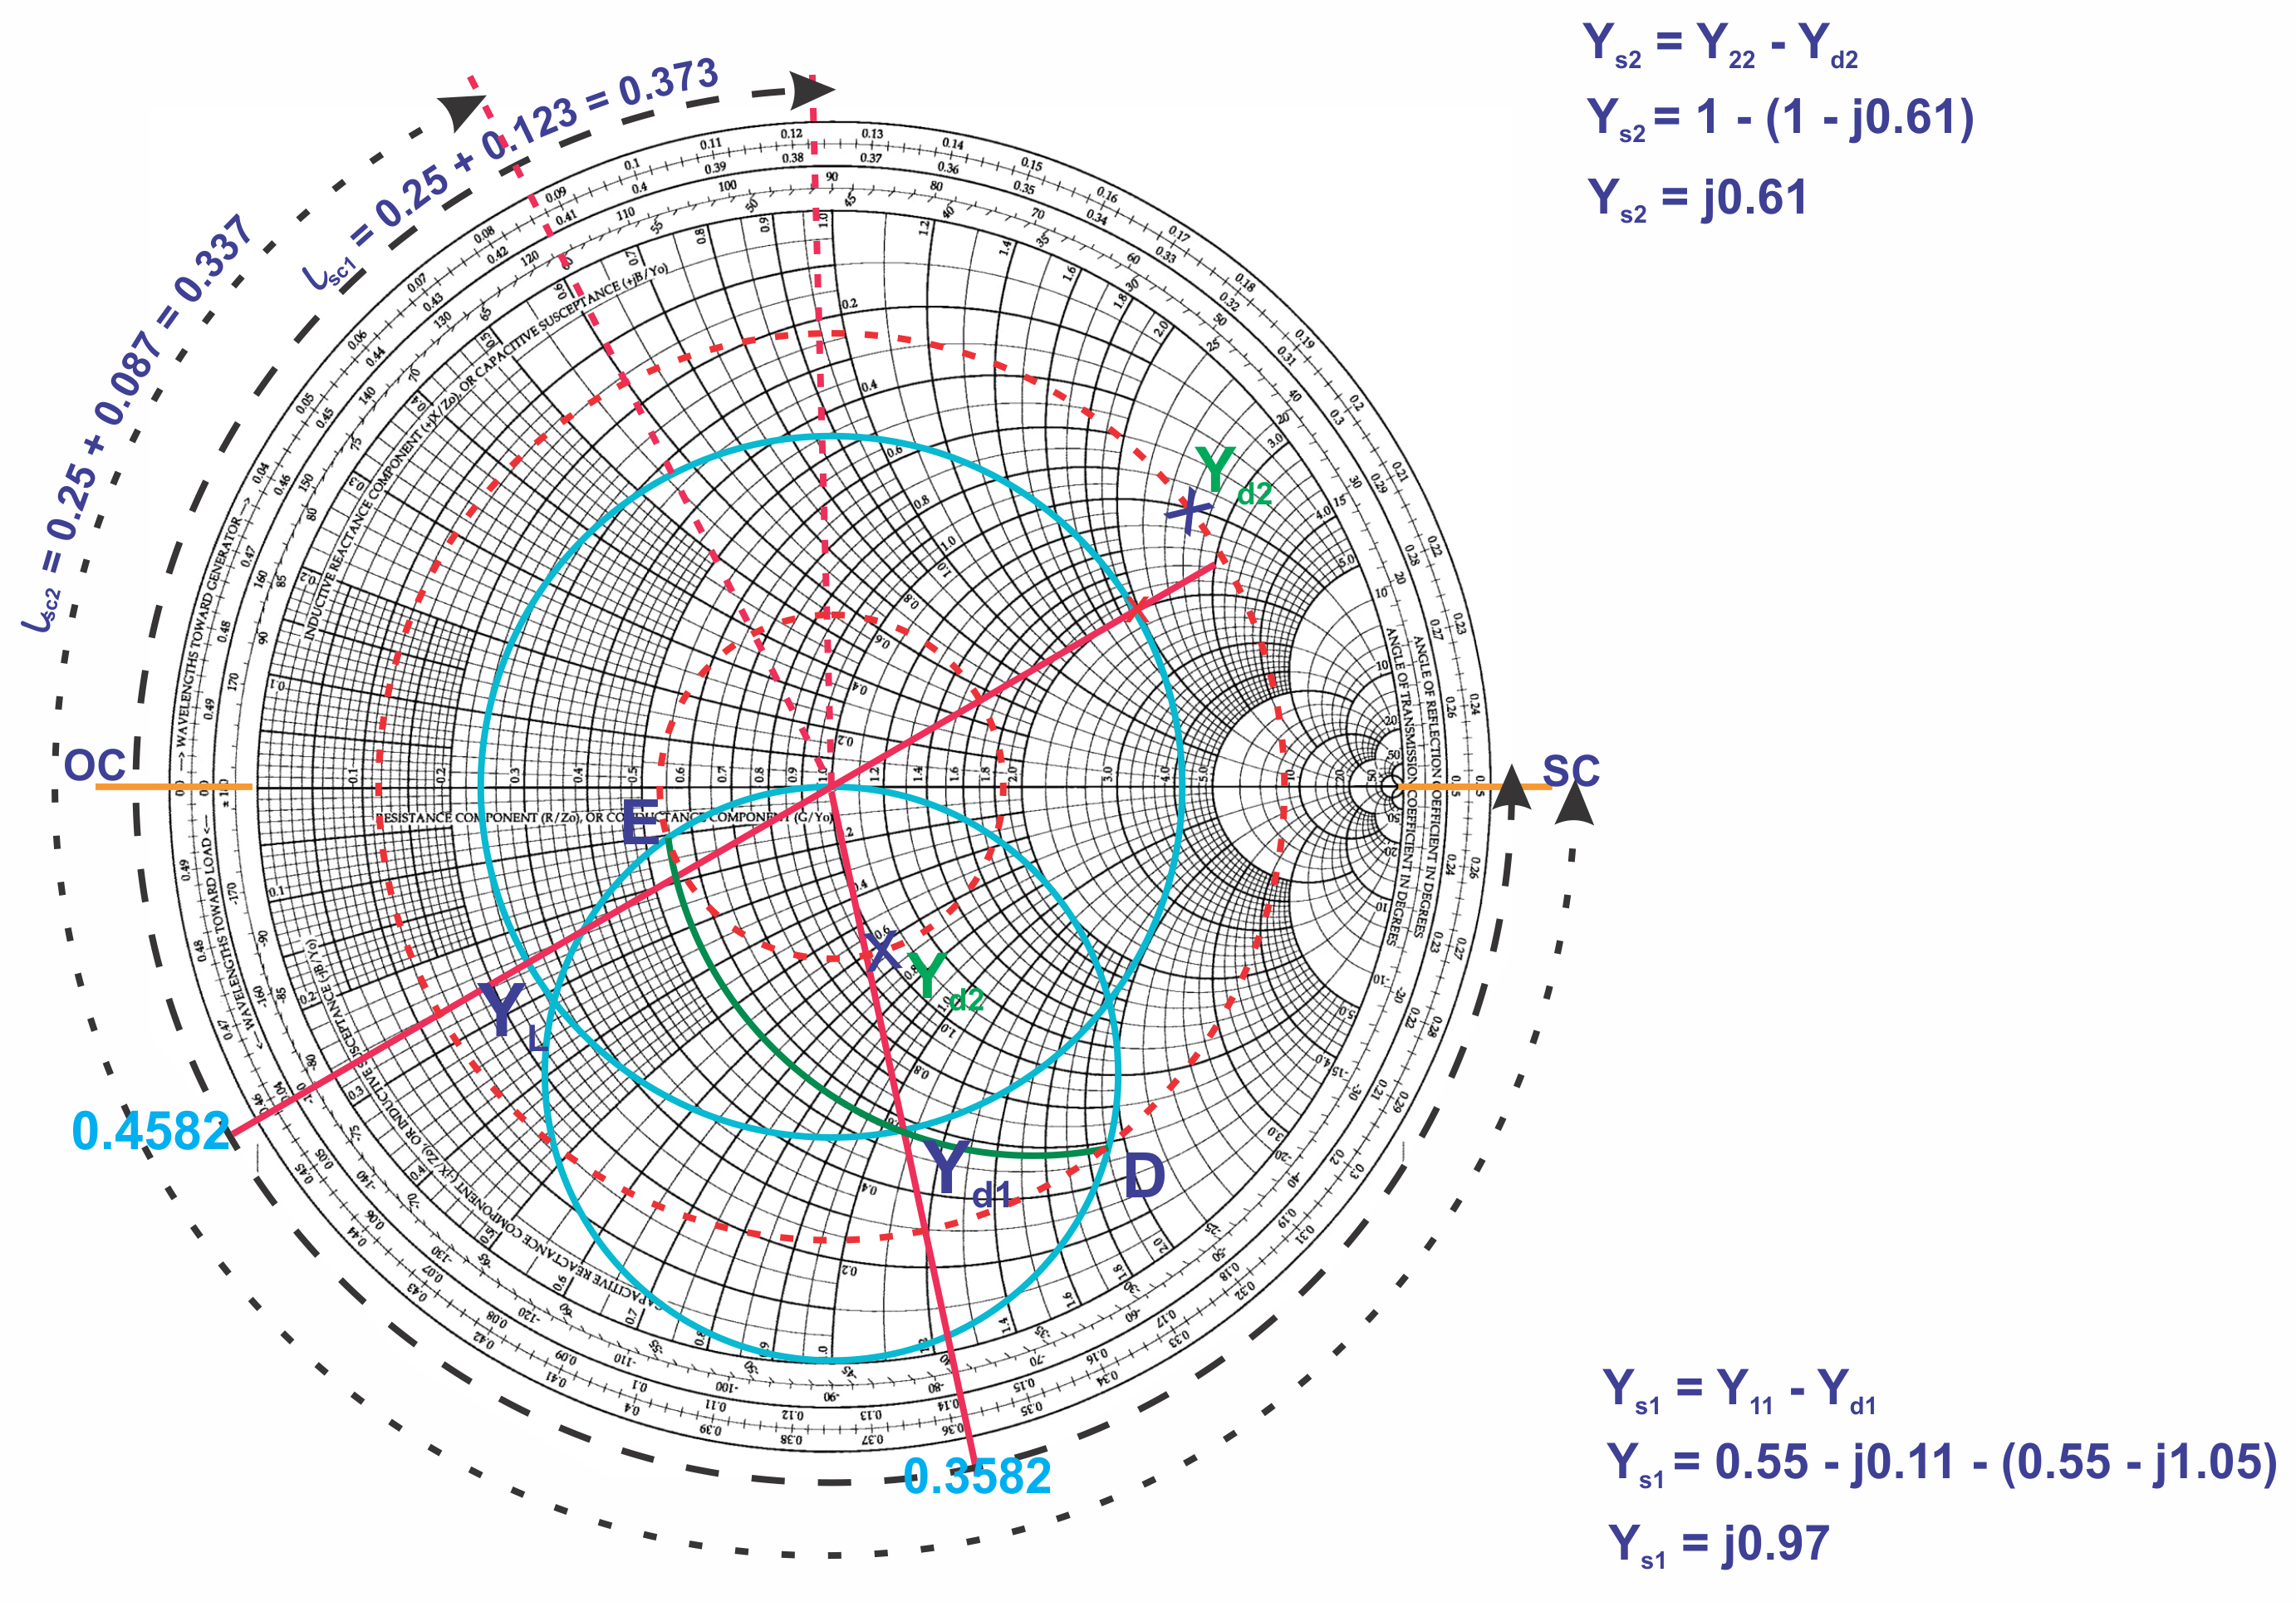
\includegraphics[width=1\linewidth]{\pathtopartone/graphics/question1}
\caption{Worked Example}
\label{fig:question1}
\end{figure}

\item Mark the point on the Smith Chart $\bar{Z_{L}} = 2 + j2$  
\item Draw the constant VSWR circle from the normalized impedance point
\item Move 180\textdegree\; from the normalized impedance point on the constant VSWR circle to the normalized admittance $Y_{L}$
\item Extend the point $Y_{L}$ to meet the bigger circle on the Smith Chart 
\item Where the line meets the VSWR circle mark the point and name it $Y_{d1}$            
\item Draw a rotated 270\textdegree\; circle of radius 1. \textbf{Note:} $\frac{3\lambda}{8}$ correspond to 270\textdegree\; rotation on the Smith Chart because $0.5\lambda$ correspond to 360\textdegree.
\item At point $Y_{d1}$, moving at constant $g$ mark point E and D which cuts the rotated 270\textdegree circle of radius 1 at point ends.
\item Point E and D are $Y_{11}$                        
\item Solve for $Y_{s1}$ (Using either point E and D as $Y_{11}$) $Y_{s1}$ =  $Y_{11}$ -  $Y_{d1}$           
\item Mark point $Y_{s1}$ on the Smith Chart, extend the point to the circle and measure its wavelength towards the generator $l^{1}$ 
\item Moving from short circuit point to point $Y_{s1}$. Calculate the distance
$ l_{s1} = 0.25 + l^{1} $                                    
\item To get $l_{s2}$. With the radius from the centre to point E, draw a circle and with the radius from the centre to point D draw a circle
\item Mark the $270\deg$ point of radius point E circle, where it meets with the unit resistance circle, mark the point and call it $Y_{d2}$. With radius from centre to point, D mark the $270\deg$ point, where it meets with the unit resistance circle and call it $Y_{d2}^{1}$ 
\item With point $Y_{d2}$ or $Y_{d2}^{1}$ get $Y_{s2}$ $Y_{22}=1$ $Y_{s2}=Y_{22}-Y_{d2}^{1}$
\item Mark the point $Y_{d2}$ on the Smith Chart and extend to the outer circle. Mark the point $l^{11}$
\item Measure the length from the short circuit point to the $l^{11}$ $Y_{d2} = 0.25 + l^{11}$
\end{enumerate}
\end{exmp}

\subsubsection{Three Stub Matching Technique}
\begin{figure}[h]
\centering
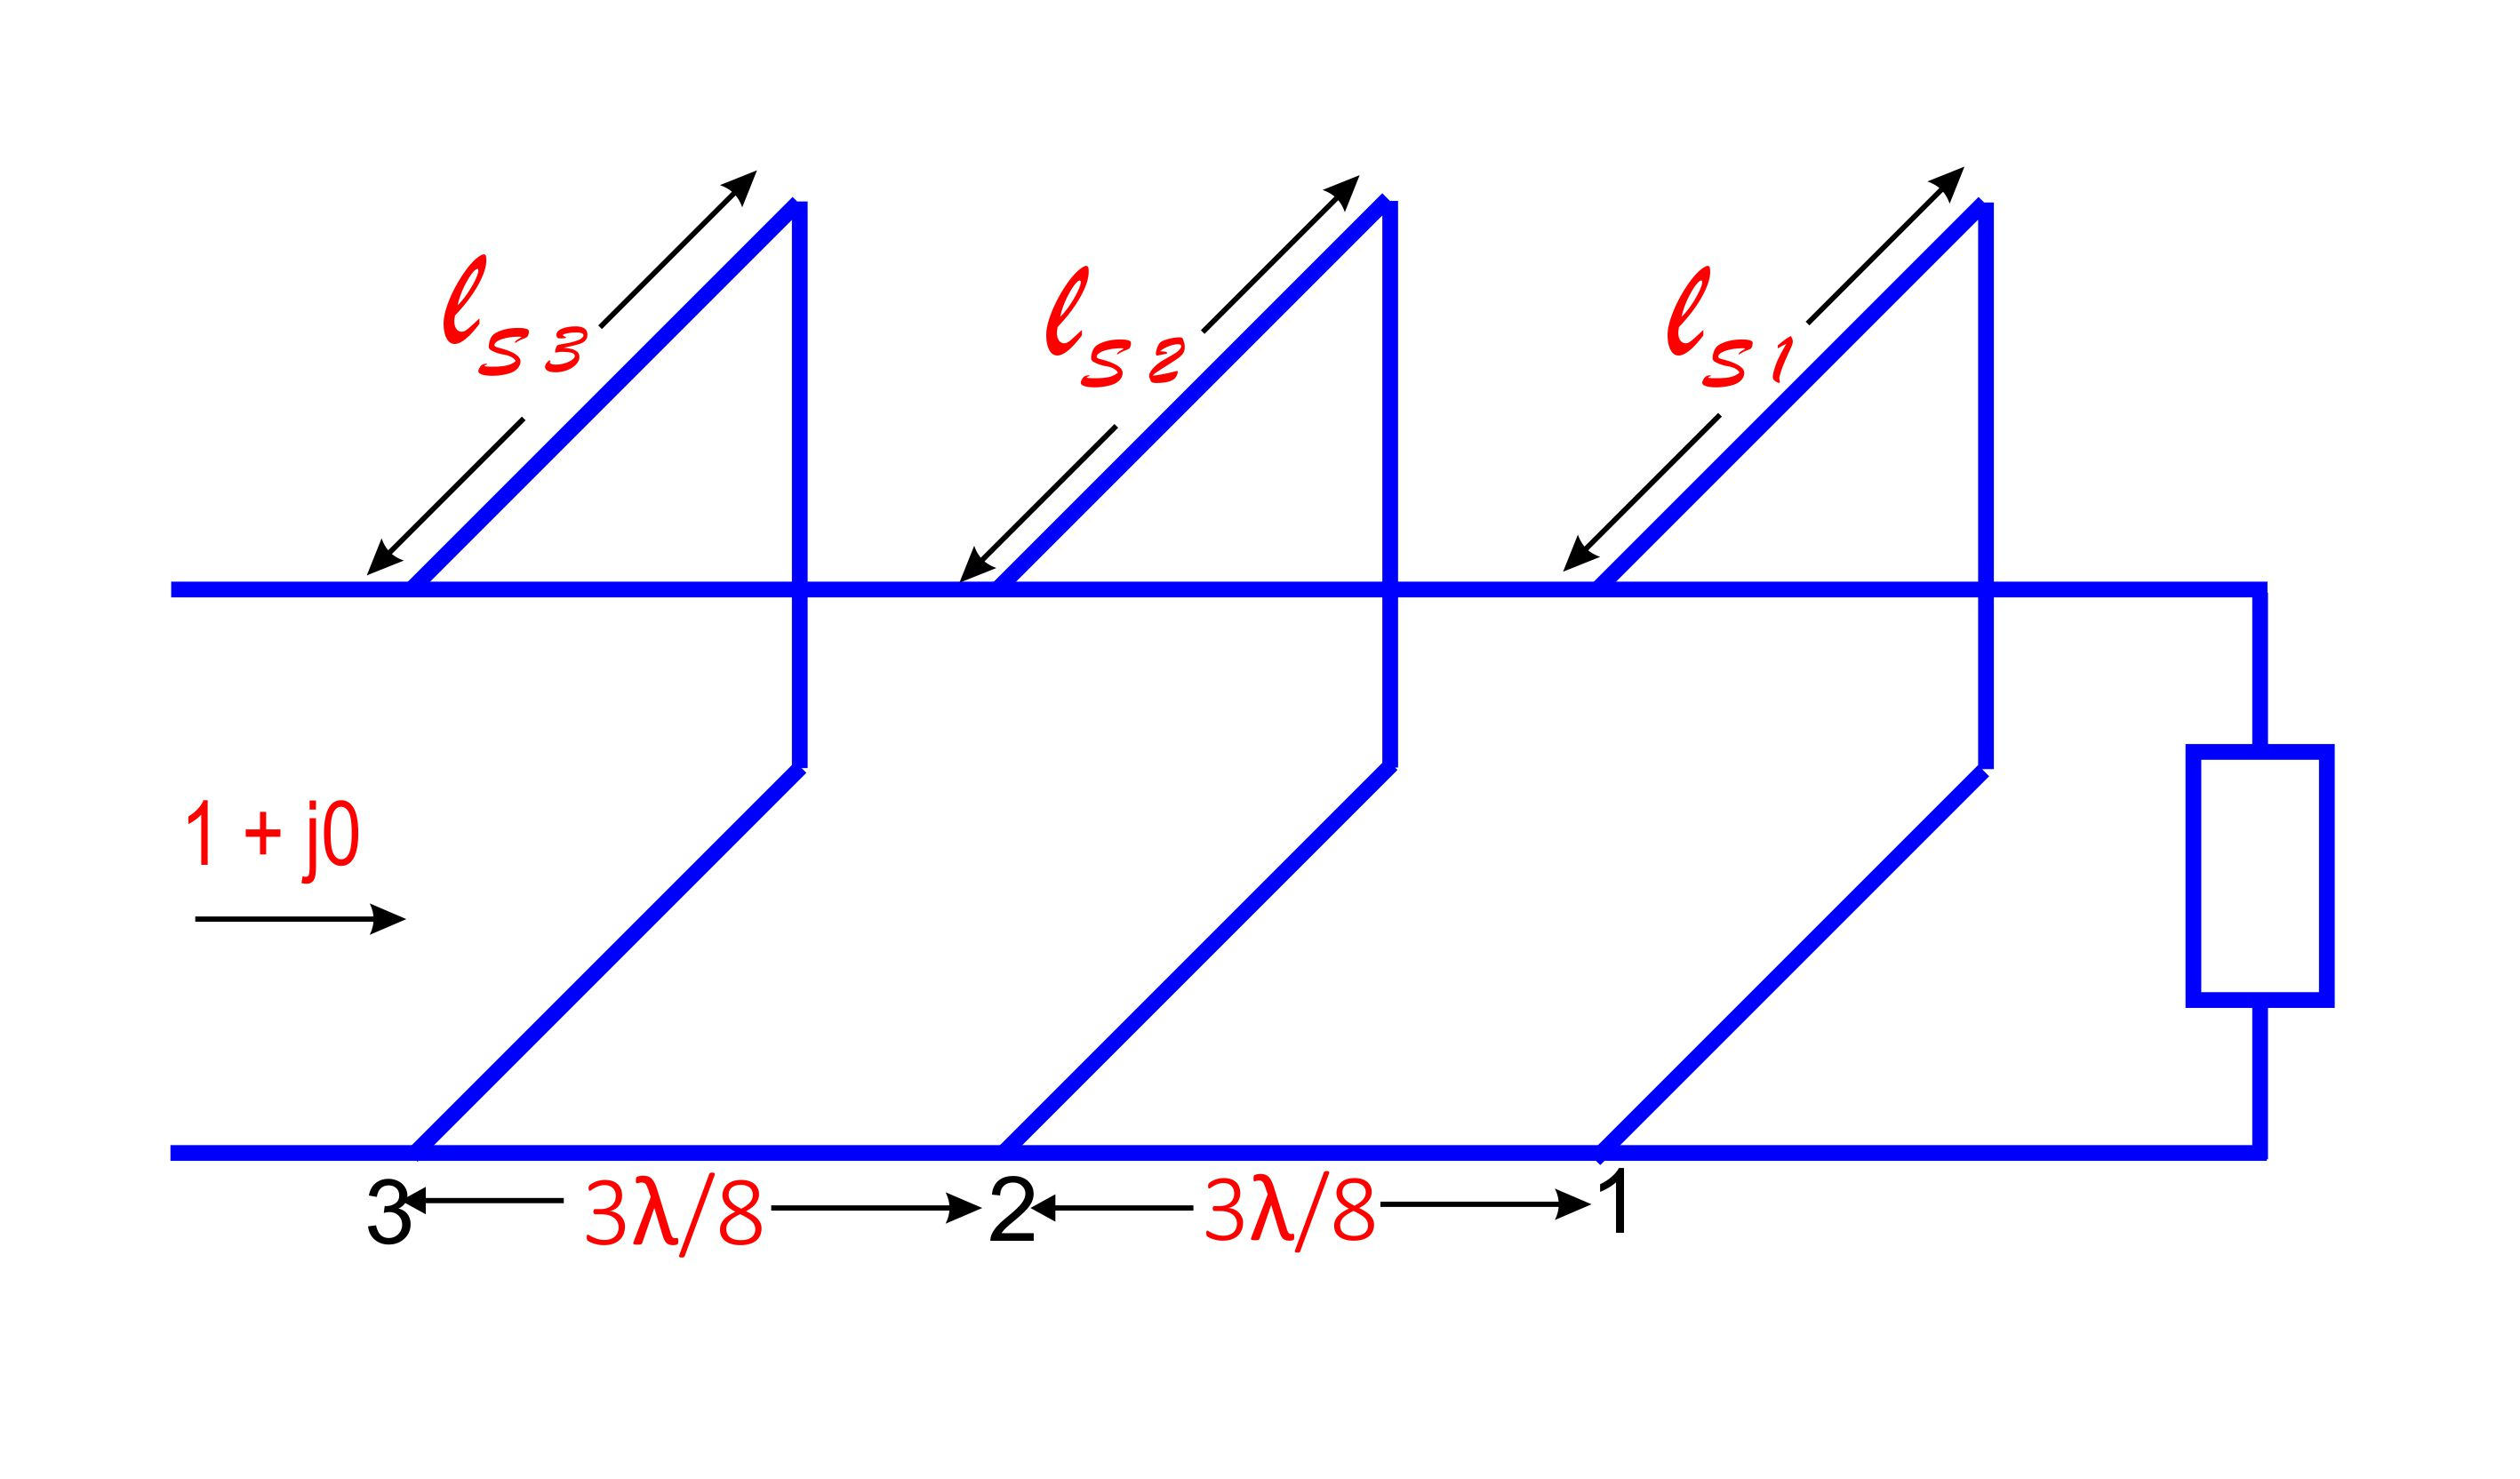
\includegraphics[width=1\linewidth]{\pathtopartone/graphics/fig13}
\caption{Three stub matching technique with three auxiliary lines attached}
\label{fig:fig13}
\end{figure}

From figure~\ref{fig:fig13}, if the matching is done with stub 2 and 1 and stub 3 is made an open circuit (so that the $ l_{s3}$ equals quarter wavelength, $\frac{\lambda}{4}$), we find that stub 2 and 3 makes the transformed impedance to lie in the forbidden region. So we disconnect stub 3 and make use of stubs 1 and 2. Depending on whether the transformed impedance lie within the forbidden region or not, we can make use of stub 1 and 2 or stub 2 and 3. The final solution for impedance matching is the three-stub technique. By using this method, all possible impedances can be matched without moving the location of the stub on the transmission line.

In conclusion, we have dealt with the major application of transmission lines which is impedance matching in which we covered the different methods with which impedance can be matched. These are:
\begin{enumerate}
\item The quarter wavelength matching technique.
\item Single stub matching technique.
\item Double stub matching technique and
\item The triple stub matching technique.
\end{enumerate}

In the end, we resolved that the triple stub matching technique is the best technique among all the techniques.

\section*{Exercises}
\begin{ExerciseList}
\Exercise[label={ex121}]
A load impedance of $Z_{L} = (100 + j100)\Omega$ is to be matched to a transmission line of characteristic impedance $Z_0 = 50\Omega$ using a double stub matching technique. The length of the line is $l_{1} = 0.4\lambda$. Determine the length of the stubs and the distance of the stubs from the load.
\Answer[ref={ex121}]
Solution to exercise~\ref{ex121}

\Exercise[label={ex122}]
A $50\varOmega$ transmission line with an air core operates at 100MHz and is connected to a load impedance of $Z_L = (27.5 + j35)\varOmega$. Design a single stub tuner.
\Answer[ref={ex122}]
Solution to exercise~\ref{ex122}

\Exercise[label={ex123}]
Find the matching network to match $Z_L = (100 + j100)\varOmega$ to a line characteristic impedance $50\varOmega$ using:
\begin{enumerate}[(a)]
\item a single series O.C stub
\item a single parallel(shunt) O.C stub
\item a single series S.C stub
\item a single parallel S.C stub
\end{enumerate}
\Answer[ref={ex123}]
Solution to exercise~\ref{ex123}

\Exercise[label={ex124}]
The terminating impedance of a transmission line, $Z_L$ is $(100 + j100)\varOmega$ and the characteristic impedance, $Z_0$ of the line is  $50\varOmega$. The first stub is placed at $0.4\lambda$ away from the load. The distance between the two stubs is $\frac{3}{8}\lambda$. Determine the length of the short-circuited shunt stubs for matching to be achieved. What terminations are forbidden for matching by the double stub?
\Answer[ref={ex124}]
Solution to exercise~\ref{ex124}

\Exercise[label={ex125}]
Determine the values of $d$ and $l$ in the single stub matching setup shown in figure~\ref{fig:singlestubproblem}.
\begin{figure}[h]
\centering
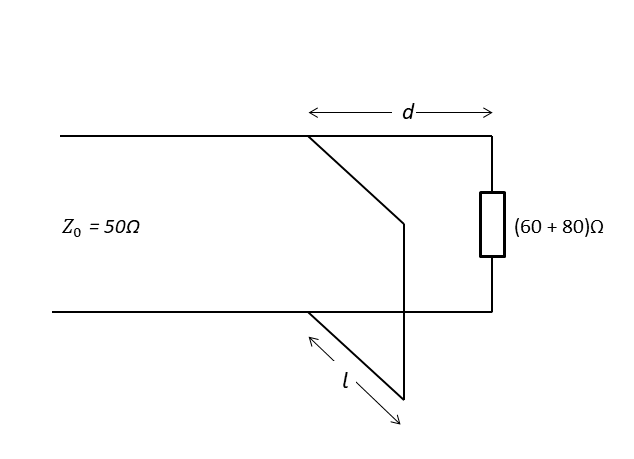
\includegraphics[width=1\linewidth]{\pathtopartone/graphics/Ex42}
\caption{Ex.~\ref{ex125}}
\label{fig:singlestubproblem}
\end{figure}
\Answer[ref={ex125}]
Solution to exercise~\ref{ex125}
\end{ExerciseList}
